%%%%%%%%%%%%%%%%%%%%%%%%%%%%%%%%%%%%%%%%%%%%
\section{The standard model}\label{sec:SMintro}
%%%%%%%%%%%%%%%%%%%%%%%%%%%%%%%%%%%%%%%%%%%%

The standard model attempts to explain all the phenomena in nature in terms of the properties and interactions of a small number of fundamental particles
of three distinct categories (Table~\ref{tab:SMparticles}): two spin-1/2 families of fermions called \textit{leptons} and \textit{quarks}, and one family of spin-1 bosons called \textit{gauge bosons},
which act as `force carriers' in the theory.
All particles of the SM are assumed to be \textit{elementary}, i.e. they are treated as point particles, without internal structure or excited states.\\

\begin{table}[!htb]
\caption{Particles of the standard model~\cite{Olive:2016xmw}.}
\label{tab:SMparticles}
\begin{center}
\begin{tabular}{r | c | c | c | c | c |}
\cline{2-6}
                               & Symbol & Name  & Mass (\MeV) & Charge ($e$) & Spin\\
 \cline{2-6}
 Up-type quarks      & $u$ & up & 2.2 & +2/3 & 1/2\\
                               & $c$ & charm & 1.27 & +2/3 & 1/2\\
                               & $t$  & top & 173.21 & + 2/3 & 1/2\\
 \cline{2-6}
 Down-type quarks & $d$ & down & 4.7 & -1/3 & 1/2\\
                               & $s$ & strange & 96 & -1/3 & 1/2\\
                               & $b$ & bottom & 4.18 & -1/3 & 1/2\\
 \cline{2-6}
 Up-type leptons    & $\nu_e$ & electron neutrino & $< 2$ eV & 0 & 1/2\\
                              & $\nu_\mu$ & muon neutrino & $< 0.19$ & 0 & 1/2\\
                              & $\nu_\tau$ & tau neutrino & $< 18.2$ & 0 & 1/2\\
 \cline{2-6}
 Down-type leptons  & $e$ & electron & 0.51 & -1 & 1/2\\
                                 & $\mu$ & muon & 105.7 & -1 & 1/2\\
                                 & $\tau$ & tau & 1776.9 & -1 & 1/2\\
 \cline{2-6}   
 Gauge bosons & $\gamma$ & photon & 0 & 0 & 1\\
                         & $\PW^\pm$ & \PW & 80.4 \GeV & $\pm 1$ & 1\\
                         & \PZ & \PZ & 91.2 \GeV & 0 & 1\\ 
                         & $g$ & gluon & 0 & 0 & 1\\          
  \cline{2-6}   
  Higgs boson & \PH & Higgs & 125.1 \GeV & 0 & 0\\
  \cline{2-6}                                           
\end{tabular}
\end{center}
\end{table}

%fermion
The class of fermions include six quarks (up, down, charm, strange, top, bottom) and six leptons (electron, electron neutrino, muon, muon neutrino, tau, tau neutrino),
which are organized in three groups (generations) of pairs from each category:
%Pairs from each category are grouped together to form a generation, with corresponding particles exhibiting similar physical behavior.

\[
\begin{pmatrix}
  \nu_e & u \\ e & d
\end{pmatrix}
\qquad
,
\qquad
\begin{pmatrix}
  \nu_\mu & c \\ \mu & s
\end{pmatrix}
\qquad
,
\qquad
\begin{pmatrix}
  \nu_\tau & t \\ \tau & b
\end{pmatrix}.
\]

The defining property of the quarks is that they carry color charge, and hence, interact via the \textit{strong interaction}.
A phenomenon called color confinement results in quarks being very strongly bound to one another, forming color-neutral composite particles (\textit{hadrons})
containing either a quark and an antiquark (\textit{mesons}) or three quarks (\textit{baryons}).
Familiar examples of baryons are the proton and neutron, which also have the smallest mass among this family of particles.
As quarks also carry electric charge and weak isospin, they interact with other fermions both via the \textit{electromagnetic and weak interactions}.
The three neutrinos do not carry electric charge, so their interaction is only driven by the weak force, which makes them difficult to detect.
However, since they carry an electric charge, the electron, muon, and tau all interact electromagnetically.
Each member of a generation has greater mass than the corresponding particles of lower generations.
As the first generation charged particles do not decay, all ordinary matter is composed of such particles.
In particular, all atoms consist of electrons orbiting around atomic nuclei, ultimately constituted of up and down quarks.
Second and third generation charged particles, on the other hand, decay with very short half lives, and are observed only in very high-energy environments.
Neutrinos of all generations also do not decay, and pervade the universe, but rarely interact with ordinary matter.
Although neutrinos were originally assumed to be massless in the standard model, it is now known from experimental results that they have very small but finite masses.
To each of these fermions is associated an anti-particle with same mass and opposite quantum numbers.

In the SM, gauge bosons are defined as force carriers that mediate the strong, weak, and electromagnetic fundamental interactions.
The use of the word `gauge' refers to the fact that all three fundamental interactions arise as consequences of requiring invariance under local gauge symmetries. 
Specifically, the gauge symmetry group of the SM is $SU(3)_C \times SU(2)_L \times U(1)_Y$.
Among the gauge bosons, the \textit{photons} mediate the electromagnetic force between electrically charged particles.
The photon is massless and is well-described by the theory of \textit{quantum electrodynamics} (QED).
The $\PW^{\pm}$ and \PZ gauge bosons mediate the weak interactions between particles of different flavors (all quarks and leptons).
They are massive, with the \PZ being slightly heavier than the \PW.
The weak interactions involving the \PW exclusively act on left-handed particles and right-handed antiparticles.
Furthermore, the \PW carries an electric charge and couples to the electromagnetic interaction.
The electrically neutral \PZ boson interacts with both left-handed particles and antiparticles.
These three gauge bosons along with the photons are grouped together, as collectively mediating the \textit{electroweak interaction}, which is described in Section~\ref{subsec:EWtheory}.

Eight massless \textit{gluons} carrying color charge, mediate the strong interactions between quarks and also interact among themselves.
The gluons and their interactions are described by the theory of \textit{quantum chromodynamics} (QCD), which is described in Section~\ref{subsec:QCD}.

As discussed in more in detail in Section~\ref{subsec:EWSB}, one additional spin-0 particle, called the \textit{Higgs boson}, is postulated to explain the origin of mass within the theory,
since without it all the particles in the model are predicted to have zero mass.

%gravity
In addition to the strong, weak and electromagnetic interactions between quarks and leptons, there is a fourth force of nature, gravity, which is not accounted for in the standard model.
In fact, the gravitational interaction between elementary particles is so small that it can be neglected at the presently accessible energies.

%%%%%%%%%%%%%%%%%%%%%%%%%%%%%%%%%%%%%%%%%%%%
\subsection{Electroweak theory}\label{subsec:EWtheory}
%%%%%%%%%%%%%%%%%%%%%%%%%%%%%%%%%%%%%%%%%%%%

The theory of electroweak interactions is based on the $SU(2)_L \times U(1)_Y$ gauge group with the quantum numbers of weak isospin $I$ and hypercharge $Y$.
Quarks and leptons are represented by spinor fields $\psi$, which are functions of continuous space-time coordinates $x^\mu$.
From experimental evidences it is known that the weak interaction is of the form of vector minus axial current ($V - A$), or in other words, it couples only to left-handed chirality states.
It is therefore convenient to write the field $\psi$ as the sum of the two chirality components:

\begin{equation}\label{eqn:SM_e1}
\psi_L(x) = \frac{1-\gamma^5}{2}\psi(x) \qquad\qquad \mbox{and} \qquad\qquad  \psi_R(x) = \frac{1+\gamma^5}{2}\psi(x).
\end{equation}

The left-handed fields are grouped into $SU(2)_L$ doublets consisting of one charged and one neutral lepton, or one up and one down quark,
with a weak isospin $I = 1/2$:

\[
\begin{pmatrix}
  \nu_\ell \\ \ell
\end{pmatrix}_L
\qquad
\mbox{and}
\qquad
\begin{pmatrix}
  q_u \\ q_d 
\end{pmatrix}_L.
\]

For up-type quarks and neutrinos the third component of the weak isospin is assigned as $I_3 = +1/2$; for down-type quarks and charged leptons the component is $I_3 = -1/2$.
The right-handed partners ($\ell_R\, ,\, q_{uR}\, ,\, q_{dR}$) transform as $SU(2)_L$ singlet with weak isospin $I_3 = 0$.
The weak hypercharge $Y$ aforementioned is then defined via electric charge $Q$ and weak isospin to be $Y = 2Q - 2I_3$.
Thus, members within a doublet carry the same hypercharge: $Y = -1$ for leptons and $Y = 1/3$ for quarks.\\

In quantum field theories, the equations of motion for the different fields considered are derived from the Lagrangian that contains all the information on the fields and on their interaction.
In the SM, the fermionic fields are added by hand to the Lagrangian to account for experimental observations.
The situation is however different for the bosonic fields, as their existence is a direct consequence of invariance properties of the Lagrangian.
This mechanism can be understood by starting from the Lagrangian for a free spin-1/2 particle with mass $m$:

\begin{equation}\label{eqn:SM_e2}
\mathcal{L}_0 = i\bar{\psi}\gamma^\mu\partial_\mu\psi - m\bar{\psi}\psi , 
\end{equation}

\noindent where $\gamma^\mu$ are the Dirac matrices.
It is straightforward to verify that the $\mathcal{L}_0$ is invariant under \textit{global} $U(1)$ transformations

\begin{equation}\label{eqn:SM_e3}
\psi(x) \xrightarrow{U(1)} \psi^\prime(x) \equiv e^{iQ\theta} \psi(x),
\end{equation}

\noindent where $Q$ is the electric charge carried by the particle involved and $\theta$ an arbitrary constant.
However, the free Lagrangian is no longer invariant if one allows the phase transformation to depend on the space-time coordinate, i.e. under local phase redefinitions $\theta = \theta(x)$, because

\begin{equation}\label{eqn:SM_e4}
\partial_\mu\psi(x) \xrightarrow{U(1)} e^{iQ\theta} (\partial_\mu + iQ\partial_\mu\theta)\psi(x),
\end{equation}

\noindent and $\mathcal{L}_0$ picks up an extra term.
The \textit{gauge invariance} is the requirement that the $U(1)$ phase invariance should hold locally.
This is only possible if some additional terms are added to the Lagrangian, so to cancel the $\partial_\mu\theta$ term in Eq.~\ref{eqn:SM_e4}.
This is achieved by introducing a new spin-1 field $A_\mu(x)$, called a ``gauge'' field, that transforms as

\begin{equation}\label{eqn:SM_e5}
A_\mu(x) \xrightarrow{U(1)} A^\prime_\mu(x) \equiv A_\mu(x) + \frac{1}{e}\partial_\mu\theta, 
\end{equation}

\noindent and by defining a covariant derivative

\begin{equation}\label{eqn:SM_e6}
\mathcal{D}_\mu \equiv \partial_\mu - ieQA_\mu,
\end{equation}

\noindent which has the required property of transforming like the field itself:

\begin{equation}\label{eqn:SM_e7}
\mathcal{D}_\mu\psi(x) \xrightarrow{U(1)} (\mathcal{D}_\mu\psi)^\prime(x) \equiv e^{iQ\theta} \mathcal{D}_\mu\psi(x).
\end{equation}

The resulting Lagrangian

\begin{equation}\label{eqn:SM_e8}
\mathcal{L} = i\bar{\psi}\gamma^\mu\mathcal{D}_\mu\psi - m\bar{\psi}\psi = \mathcal{L}_0 + eQA_\mu\bar{\psi}\gamma^\mu\psi
\end{equation}

\noindent is then invariant under local $U(1)$ transformations.
For the new gauge field to be a true propagating field, a gauge-invariant kinetic term has to be added to the Lagrangian

\begin{equation}\label{eqn:SM_e9}
\mathcal{L}_A = -\frac{1}{4}F_{\mu\nu}F^{\mu\nu},
\end{equation}

\noindent where $F_{\mu\nu} \equiv \partial_\mu A_\nu - \partial_\nu A_\mu$. 
A possible mass term for the gauge field, $m^2A^\mu A_\mu$, is forbidden because it would violate gauge invariance,
so that it is predicted to be massless.
The new gauge field can be easily identified with the electromagnetic potential,
and the total Lagrangian 

\begin{equation}\label{eqn:SM_e10}
\mathcal{L} = \left[ i\bar{\psi}\gamma^\mu\partial_\mu\psi - m\bar{\psi}\psi \right] + \left[ -\frac{1}{4}F_{\mu\nu}F^{\mu\nu} \right] + [eQA_\mu\bar{\psi}\gamma^\mu\psi]
\end{equation}

\noindent gives rise to the well-known Maxwell equations of the electrodynamics

\begin{equation}\label{eqn:SM_e11}
\partial_\mu F^{\mu\nu} = J^\nu \, , \qquad\qquad J^\nu = -eQ\bar{\psi}\gamma^\nu\psi,
\end{equation}

\noindent where $J^\nu$ is the fermion electromagnetic current.
Thus, the final Lagrangian in Eq.~\ref{eqn:SM_e10} represents the final expression for the Lagrangian of quantum electrodynamics,
describing Dirac fields (fermions) interacting wth Maxwell fields (photons).\\

To describe weak interactions, a more elaborated structure is needed, with several fermionic flavors and different properties for left- and right-handed fields.
Moreover, the left-handed fermions must appear in doublets, and massive gauge bosons $\PW^{\pm}$ and $\PZ$ must be present in addition to the photon.
The simplest group with doublet representations is $SU(2)$, and since the theory must include QED as well, the additional $U(1)$ group is needed.
Hence, the obvious symmetry group to consider is $SU(2)_L \times U(1)_Y$, where $L$ refers to left-handed fields and $Y$ to the hypercharge.

The free Lagrangian for a generation of quarks (or leptons) is given by

\begin{equation}\label{eqn:SM_e12}
\mathcal{L}_0 = \sum_{j=1}^3 i\bar{\psi}_j\gamma^\mu\partial_\mu\psi_j,
\end{equation}

\noindent where the following notation has been introduced

\begin{equation}\label{eqn:SM_e13}
\psi_1(x) = 
\begin{pmatrix}
  u \\ d
\end{pmatrix}_L
\,
,
\qquad
\psi_2(x) = u_R \, , \qquad \psi_3(x) = d_R.
\end{equation}

The free Lagrangian $\mathcal{L}_0$ is invariant under global $G$ transformations in flavor space:

\begin{equation}\label{eqn:SM_e14}
\begin{split}
\psi_1(x) & \xrightarrow{G} \psi_1^\prime(x) \equiv e^{iY_1\beta}U_L\psi_1(x) \\ 
\psi_2(x) & \xrightarrow{G} \psi_2^\prime(x) \equiv e^{ig^\prime Y_2\beta}\psi_2(x) \\
\psi_3(x) & \xrightarrow{G} \psi_3^\prime(x) \equiv e^{ig^\prime Y_3\beta}\psi_3(x)
\end{split}
\end{equation}

\noindent where the $SU(2)_L$ transformation

\begin{equation}\label{eqn:SM_e15}
U_L \equiv e^{ig\frac{\tau^i}{2}\alpha^i} \qquad\qquad (i = 1,2,3)
\end{equation}

\noindent only acts on the doublet field $\psi_1$.
%The parameters $Y_i$ are the hypercharges, since the $\mathrm{U(1)_Y}$ phase transformation is analog to the QED one.
The parameters $Y_i$ are three different values (one per each field) of the hypercharge, which represents the generator of the symmetry group $U(1)_Y$.
The $\beta$ parameter is the phase of the $U(1)_Y$ transformation and is one-dimensional.
The matrices $\tau_i$ are the Pauli matrices and represent the three $SU(2)_L$ transformation generators which are combined in the weak isospin operator
$\textbf{T} = (\tau_1, \tau_2, \tau_3)$. These matrices form a Lie group, which is defined by the commutator relation $[\tau_i,\tau_j] = i\epsilon_{ijk}\tau_k$.
As the $\tau_i$ do not commute, the $SU(2)_L$ group is called non-Abelian.
%The matrix transformation UL is non-abelian.
Due to the generator structure, the phase $\alpha = (\alpha_1, \alpha_2, \alpha_3)$ of the $SU(2)_L$ transformation has to be extended to a three-component vector with the same dependencies as above.
The couplings $g$ and $g^\prime$ have been introduced for the $SU(2)_L$ and $U(1)_Y$, respectively, quantifying the strength of the interactions.

The free Lagrangian in Eq.~\ref{eqn:SM_e12} is then required to be invariant under local $SU(2)_L\times U(1)_Y$ gauge transformations,
i.e. with $\alpha_i = \alpha_i(x)$ and $\beta = \beta(x)$.
In order to satisfy this symmetry requirement, the fermion derivatives are exchanged with covariant objects.
Since there are now four gauge parameters, $\alpha_i(x)$ and $\beta(x)$, four different gauge fields are needed:

\begin{eqnarray}\label{eqn:SM_e16}
\mathcal{D}_\mu \equiv \partial_\mu + ig\textbf{W}_\mu \cdot \textbf{T} + ig^\prime\frac{Y}{2}B_\mu.
%\mathcal{D}_\mu \equiv \partial_\mu + ig\frac{\tau_i}{2}W^i_\mu + ig^\prime\frac{Y}{2}B_\mu.
\end{eqnarray}

Thus, four additional vector fields of spin 1 have been added: the isotriplet $\textbf{W}_\mu = (W_{1\mu}, W_{2\mu}, W_{3\mu})$ for the $SU(2)_L$ and the singlet $B_\mu$ for the $U(1)_Y$.
The quanta of these fields are called gauge bosons.
In order to build the gauge-invariant kinetic term for the gauge bosons, the corresponding field strengths are introduced: 

\begin{equation}\label{eqn:SM_e17}
\begin{split}
B_{\mu\nu} & \equiv \partial_\mu B_\nu - \partial_\nu B_\mu\\
W^i_{\mu\nu} & \equiv \partial_\mu W^\prime_\nu - \partial_\nu W^i_\mu - g\epsilon_{ijk} W^j_\mu W^k_\nu.
\end{split}
\end{equation}

The final $SU(2)_L \times U(1)_Y$ Lagrangian is then given by

\begin{equation}\label{eqn:SM_e18}
\mathcal{L}_{SU(2)_L\times U(1)_Y} = \mathcal{L}_f + \mathcal{L}_g,
\end{equation}

\noindent where $\mathcal{L}_f$ is the Lagrangian for the free fermion fields

\begin{equation}\label{eqn:SM_e19}
\mathcal{L}_f = i\sum_{j}\bar{\psi}^j_L\gamma^\mu[\partial_\mu + ig\textbf{W}_\mu \cdot \textbf{T} + ig^\prime\frac{Y_L}{2}B_\mu]\psi^i_L + i\sum_j\bar{\psi}^j_R[\partial_\mu - g^\prime Y_RB_\mu]\psi^j_R
\end{equation}

\noindent and $\mathcal{L}_g$ is the Lagrangian for the gauge bosons

\begin{equation}\label{eqn:SM_e20}
\mathcal{L}_g = -\frac{1}{4}\textbf{W}_{\mu\nu} \cdot \textbf{W}^{\mu\nu} - \frac{1}{4}B_{\mu\nu} \cdot B^{\mu\nu}.
\end{equation}

Since the field strengths $W^i_{\mu\nu}$ contain a quadratic term, the Lagrangian $\mathcal{L}_g$ gives rise to cubic and quartic self-interactions among the gauge fields.
The strength of these interactions is given by the same $SU(2)_L$ coupling $g$ which appears in the fermionic piece of the Lagrangian.
The final Lagrangian represents the unified electroweak theory, developed by Glashow~\cite{GLASHOW1961579}, Weinberg~\cite{PhysRevLett.19.1264} and Salam~\cite{RevModPhys.52.525}.
However, this is not the entire theory since the gauge symmetry forbids to write a mass term for the gauge bosons.
Fermionic masses are also not possible, because they would connect the left- and right-handed fields, which have different transformation properties, and therefore would produce an explicit breaking of the gauge symmetry.
Thus, the $SU(2)_L\times U(1)_Y$ Lagrangian in Eq.~\ref{eqn:SM_e17} only contains massless fields.
The mass terms are introduced through a procedure that exploits spontaneous symmetry breaking as described in the following.
%TF1* f = new TF1("f","-500*x*x+5*x*x*x*x",-15,15)
%TF1* f = new TF1("f","x*x",-10,10)
%TF3* f3 = new TF3("f3","x*x+y*y-z",-10,10,-10,10,0,1000)
%TF3* f3 = new TF3("f3","-500*(x*x+y*y)+5*(x*x+y*y)^2-z",-10,10,-10,10,-15000,0)

%%%%%%%%%%
\subsection{Spontaneous symmetry breaking}\label{subsec:EWSB}
%%%%%%%%%%

In order to generate masses, the gauge symmetry needs to be broken in such way to maintain the full symmetry of the Lagrangian.
The main idea is based on the possibility to obtain non-symmetric results from a Lagrangian that possess the following properties:
it is invariant under a group $G$ of transformations and has a degenerate set of states with minimal energy, which transform under $G$ as the members of a given multiplet.
As it will be demonstrated in the following, by arbitrary selecting one of those states as the ground state of the system, one says that the symmetry becomes spontaneously broken.
%The idea is that the lowest energy (vacuum) state does not respect the gauge symmetry and induces effective masses for particles propagating through it.

In order to explain this mechanism the Lagrangian for a complex scalar field $\phi(x) = \phi_1(x) + i\phi_2(x)$ is considered

\begin{equation}\label{eqn:SM_e21}
\mathcal{L} = \partial_\mu\phi^\dag\partial^\mu\phi - V(\phi) \, , \qquad\qquad V(\phi) = \mu^2\phi^\dag\phi + h(\phi^\dag\phi)^2
\end{equation}

\noindent where $V(\phi)$ is a potential. 
The Lagrangian $\mathcal{L}$ is invariant under global phase transformations of the scalar field

\begin{equation}\label{eqn:SM_e22}
\phi(x) \xrightarrow{U(1)} \phi^\prime(x) \equiv e^{i\theta} \phi(x).
\end{equation}

In order to allow for a minimum or ``ground state'' of the potential, the parameter $h$ has to be $\geq 0$. For the quadratic term there are the two following possibilities.
If $\mu^2 \geq 0$, the potential acquires only the trivial minimum $\phi_m = 0$. If $\mu^2 \leq 0$ the minimum is obtained for all those field configurations satisfying

\begin{equation}\label{eqn:SM_e23}
|\phi_m| = \sqrt{\frac{-\mu^2}{2h}} \equiv \frac{v}{\sqrt{2}} \geq 0 \qquad\qquad \Rightarrow \qquad\qquad V(\phi_m) = -\frac{h}{4}v^4
\end{equation}

As the Lagrangian is invariant under $U(1)$ phase transformations, there is an infinite number of degenerate states of minimum energy given by 
$\phi_m(x) = \frac{v}{\sqrt{2}}e^{i\theta}$.
A particular solution can be chosen, e.g. $\theta = 0$, corresponding to the minimum of the field given by $\phi_{1m} = v/\sqrt{2}$ and $\phi_{2m} = 0$.
Since the Feynman calculus is a perturbation procedure, in which starting from a ground state the fields are treated as fluctuations about that state,
two new real fields $\eta(x)$ and $\xi(x)$ are introduced representing these fluctuations

\begin{equation}\label{eqn:SM_e24}
\eta(x) = \phi_1(x) - \frac{v}{\sqrt{2}} \qquad\qquad \mbox{and} \qquad\qquad \xi(x) = \phi_2(x).
\end{equation}

In terms of these new fields, the potential $V(\phi)$ takes the form

\begin{equation}\label{eqn:SM_e25}
V(\phi) = V(\phi_m) - \mu^2\eta^2 + hv\eta(\eta^2+\xi^2) + \frac{h}{4}(\eta^2+\xi^2)^2
\end{equation}

\noindent and the resulting Lagrangian does not share the same symmetry of the original one. Thus, by choosing a particular solution as the ground state, the symmetry gets spontaneously broken.
At the same time, the second term of the potential in Eq.~\ref{eqn:SM_e25} is a mass term, so the real field $\eta$ describes a massive state of mass $m_\eta = -2\mu^2$.
The second real field $\xi$ is massless, and its appearance can be understood as follows.
The field $\xi$ describes excitations around a flat direction in the potential, i.e. into states with the same energy as the chosen ground state.
Since those excitations do not cost any energy, they correspond to a massless state.
The fact that there are massless excitations associated with the spontaneous symmetry breaking mechanism is a general result, known as the \textit{Goldstone theorem}:
if a Lagrangian is invariant under a continuous symmetry group $G$, but the vacuum is only invariant under a subgroup $H \subset G$,
then there must exist as many massless spin-0 particles (\textit{Goldstone bosons}) as broken generators (i.e. generators of $G$ which do not belong to $H$).\\

%%%%%%%%%%%%%%%%%%%%%%%%%%%%%%%%%%%%%%
\subsection{The Higgs mechanism}\label{subsec:HiggsMech}
%%%%%%%%%%%%%%%%%%%%%%%%%%%%%%%%%%%%%%

The mechanism of spontaneous symmetry breaking described in the previous section does not account for the mass of the gauge fields of the weak interaction,
since it introduces an additional massless scalar boson that is not included in the set of the known elementary particles.
However, further elements are added to the theory  when applying the idea of spontaneous symmetry breaking to the case of local gauge invariance.
In order to achieve this, the complex scalar field $\phi(x)$ introduced in the previous section is replaced with a $SU(2)_L$ doublet of complex scalar fields with $U(1)$ hypercharge $Y = +1/2$:

\begin{equation}\label{eqn:SM_e26}
\phi(x) \equiv
\begin{pmatrix}
  \phi^+(x) \\ \phi^0(x)
\end{pmatrix}
= \frac{1}{\sqrt{2}}
\begin{pmatrix}
  \phi_1(x) - i\phi_2(x) \\ \phi_3(x) - i\phi_4(x)
\end{pmatrix}.
\end{equation}

The gauged scalar Lagrangian of the Goldstone model (Eq.~\ref{eqn:SM_e21}) is now given by

\begin{equation}\label{eqn:SM_e27}
\begin{aligned}
\mathcal{L}_\phi  & = \mathcal{D}_\mu\phi^\dag\mathcal{D}^\mu\phi - \mu^2\phi^\dag\phi + h(\phi^\dag\phi)^2 \, , & \qquad (h \geq 0, \mu^2 \leq 0) \, , \\
 \mathcal{D}^\mu\phi & =  [\partial^\mu + ig\textbf{W}_\mu \cdot \textbf{T} + ig^\prime\frac{Y}{2}B_\mu] \, , & \qquad (Y = Q - \tau_3 = \frac{1}{2}) \, , 
\end{aligned}
\end{equation}

\noindent and it is invariant under local $SU(2)_L \times U(1)_Y$ transformations.
The value of the scalar hypercharge is fixed by the requirement of having the correct couplings between $\phi(x)$ and $B_\mu(x)$, i.e. that the photon does not couple to $\phi^0$, and one has the right electric charge for $\phi^+$.
As observed in the previous section, there is an infinite set of degenerate states with minimum energy satisfying

\begin{equation}\label{eqn:SM_e29}
\begin{aligned}
\left\langle0|\phi_i|0\right\rangle & = 0 \quad \mbox{for} \quad i = 1,2,4\\
\left\langle0|\phi_3|0\right\rangle & = \sqrt{\frac{-\mu^2}{2h}} \equiv \frac{v}{\sqrt{2}}.
\end{aligned}
\end{equation}

Since the electric charge is a conserved quantity, only the neutral scalar field can acquire a vacuum expectation value.
Once a particular ground state is chosen, the $SU(2)_L\times U(1)_Y$ symmetry gets spontaneously broken.
%to the electromagnetic subgroup $\mathrm{U(1)_{QED}}$, which by construction still remains a true symmetry of the vacuum. According to Goldstone theorem 3 massless states should then appear.
On the other hand, the vacuum carries no electric charge, so the $U(1)_{Q}$ of QED is not broken.
Thus, the $SU(2)_L\times U(1)_Y$ group of the electroweak theory is spontaneously broken to the $U(1)_{Q}$ subgroup, i.e. $SU(2)_L \times U(1)_Y \rightarrow U(1)_Q$.

The scalar doublet can now be written in its general, gauge-invariant form as a fluctuation over the ground state

\begin{equation}\label{eqn:SM_e30}
\phi(x) = e^{i\frac{\tau^i}{2}\theta^i(x)}\frac{1}{\sqrt{2}}
\begin{pmatrix}
  0 \\ v + H(x)
\end{pmatrix}
\end{equation}

\noindent with 4 real fields $\theta^i(x)$ and $H(x)$.
The crucial point is that the local $SU(2)_L$ invariance of the Lagrangian allows one to rotate away any dependence on $\theta^i(x)$.
These three fields would be precisely the massless Goldstone bosons associated with the spontaneous symmetry breaking mechanism.
The additional ingredient of gauge symmetry makes these massless excitations unphysical.
%The covariant derivative in Eq.~\ref{eqn:SM_e28} couples the scalar multiplet to the $\mathrm{SU(2)_L\times U(1)_Y}$ gauge bosons.
In fact, it can be demonstrated that by choosing the physical (unitary) gauge $\theta^i(x) = 0$, the 3 massless Goldstone bosons
arising from the three broken generators can be eliminated from the Lagrangian.
At the same time, the kinetic piece of the scalar Lagrangian in Eq.~\ref{eqn:SM_e27} takes the form

\begin{equation}\label{eqn:SM_e31}
(\mathcal{D}_\mu\phi)^\dag\mathcal{D}^\mu\phi \xrightarrow{\theta^i = 0} \frac{1}{2}\partial_\mu H\partial^\mu H + (v+H)^2 \left\{ \frac{g^2}{4}W^\dag_\mu W^\mu + \frac{g^2}{8\cos^2\theta_W}Z_\mu Z^\mu \right\}.
\end{equation}

The vacuum expectation value of the neutral scalar has generated a quadratic term, i.e. mass terms, for the gauge bosons.
Usually, one rewrites the fields in terms of the three massive vector bosons $\PW^\pm$ and \PZ, and a massless vector boson, the photon $A$.
One finds that they are mixtures of the original gauge fields $\mathbf{W}_\mu$ and $B_\mu$:

\begin{equation}\label{eqn:SM_e32}
W^\pm_\mu = \frac{(W^1_\mu \mp iW^2_\mu)}{\sqrt{2}},
\end{equation}

\begin{equation}\label{eqn:SM_e33}
\begin{pmatrix}
  A_\mu \\ Z_\mu
\end{pmatrix}
=
\begin{pmatrix}
  \cos\theta_W & \sin\theta_W \\ -\sin\theta_W & \cos\theta_W
\end{pmatrix}
\begin{pmatrix}
  B_\mu \\ W^3_\mu
\end{pmatrix}
\end{equation}

\noindent where the Weinberg angle $\theta_W$ is defined as the ratio of coupling constants: $\tan\theta_W \equiv g^\prime/g$.
The masses of the gauge bosons $\PW^\pm$ and the \PZ are then given by:

\begin{equation}\label{eqn:SM_e34}
M_\PW = \frac{1}{2}vg \qquad\qquad \mbox{and} \qquad\qquad M_\PZ = \frac{v\sqrt{g^2 + g^{\prime 2}}}{2} = \frac{M_\PW}{\cos\theta_W}.
\end{equation}

The Lagrangian $\mathcal{L}_\phi$ has to be added to the electroweak theory given by the Lagrangian of Eqs.~\ref{eqn:SM_e18}--\ref{eqn:SM_e20}, such that

\begin{equation}\label{eqn:SM_e35}
\mathcal{L}_{SU(2)_L \times U(1)_Y} = \mathcal{L}_f + \mathcal{L}_g + \mathcal{L}_\phi.
\end{equation}

The total Lagrangian is invariant under gauge transformations, which guarantees the renormalizability of the associated quantum field theory.
After spontaneous symmetry breaking, three massless Goldstone bosons are generated, however, they are then eliminated from the Lagrangian by exploiting local gauge symmetry.
Going to the unitary gauge, the $\PW^\pm$ and the \PZ (but not the photon, because $U(1)_Q$ is an unbroken symmetry) have acquired masses given by Eq.~\ref{eqn:SM_e34}.
%Notice that (3.22) has now the meaning of writing the gauge fields in terms of the physical boson fields with definite mass.
In fact, before the spontaneous symmetry breaking mechanism, the massless $\PW^\pm$ and \PZ bosons lead to $3\times2 = 6$ degrees of freedom (d.o.f.), due to the two possible polarizations of a massless spin-1 field.
The four real scalar fields are also present at this stage, corresponding to additional four d.o.f.
After spontaneous symmetry breaking, the three Goldstone modes are ``eaten'' by the weak gauge bosons, which become massive, and therefore acquire one additional longitudinal polarization.
This leads to a total of $3 \times 3 = 9$ d.o.f. in the gauge sector, plus the remaining scalar particle $H$, which is called the \textit{Higgs boson}. The total number of d.o.f. is obviously conserved.
This theory is generally called the \textit{Higgs mechanism} and it was proposed by three independent groups in 1964: by Brout and Englert~\cite{PhysRevLett.13.321}, by Higgs~\cite{Higgs1964132,PhysRevLett.13.508,PhysRev.145.1156}, and by Guralnik, Hagen, and Kibble~\cite{PhysRevLett.13.585}.

The W and Z were discovered at CERN by the UA1~\cite{ARNISON1986484} and UA2~\cite{ANSARI1987440} groups in 1983.
Subsequent measurements of their masses and other properties at Tevatron and LEP have been in excellent agreement with the standard model expectations~\cite{Schael:2013ita,Aaltonen:2013iut}. The current values are $M_\PW = 80.385 \pm 0.015\GeV$ and $M_\PZ = 91.1876 \pm 0.0021\GeV$~\cite{Olive:2016xmw}.

%%%%%%%%%%%%%%%%%%%%%%%%%%%%%%%%%%%%%%
\subsection{The Higgs and Yukawa interactions}\label{subsec:HiggsBoson}
%%%%%%%%%%%%%%%%%%%%%%%%%%%%%%%%%%%%%%

The scalar Lagrangian in Eq.~\ref{eqn:SM_e27} has introduced a new scalar particle into the model: the Higgs boson H.
In terms of the physical fields (unitary gauge), $\mathcal{L}_\phi$ takes the form

\begin{equation}\label{eqn:SM_e36}
\mathcal{L}_\phi = \frac{1}{4}hv^4 + \mathcal{L}_H + \mathcal{L}_{HG^2}, 
\end{equation}

\noindent where

\begin{equation}\label{eqn:SM_e37}
\begin{gathered}
\mathcal{L}_H = \frac{1}{2}\partial_\mu H\partial^\mu H - \frac{1}{2}M^2_HH^2 -\frac{M^2_H}{2v}H^3 -\frac{M^2_H}{8v^2}H^4 \, , \\
\mathcal{L}_{HG^2} = M^2_WW^\dag_\mu W^\mu \left\{ 1 + \frac{2}{v}H + \frac{H^2}{v^2} \right\} + \frac{1}{2}M^2_ZZ_\mu Z^\mu \left\{ 1 + \frac{2}{v}H + \frac{H^2}{v^2} \right\} \, ,
\end{gathered}
\end{equation}

\noindent and the Higgs boson mass is given by

\begin{equation}\label{eqn:SM_e38}
M_H = \sqrt{-2\mu^2} = \sqrt{2h}v.
\end{equation}
 
A fermionic mass term $-m\bar{\psi}\psi$ is not allowed, because it breaks the gauge symmetry.
%However, since an additional scalar doublet has been added into the model, one can write the following gauge-invariant fermion-scalar couplings:
However, by adding Yukawa interaction terms of the fermion and Higgs field to the Lagrangian, the fermion masses can also be generated by spontaneous symmetry breaking.
This procedure is briefly described in the following.
%Similarly, this applies for quarks. 

The most general Yukawa Lagrangian can be written in the form

\begin{equation}\label{eqn:SM_e39}
\sum_{jk}\left\{
(\bar{u}^\prime_j , \bar{d}^\prime_j)_L
\left[
c^{(d)}_{jk}
\begin{pmatrix}
  \phi^+ \\ \phi^0
\end{pmatrix}
d^\prime_{kR} + c^{(u)}_{jk}
\begin{pmatrix}
  \phi^{0*} \\ -\phi^-
\end{pmatrix}
u^\prime_{kR}
\right]
+ (\bar{\nu}^\prime_j , \bar{\ell}^\prime_j) c^{(\ell)}_{jk}
\begin{pmatrix}
  \phi^+ \\ \phi^0
\end{pmatrix}
\ell^\prime_{kR}
\right\} + h.c.
\end{equation}

\noindent where the indexes run over the three generations of fermions;
$u^\prime_j$, $d^\prime_j$, $\ell^\prime_j$ and $\nu^\prime_j$ denote the weak eigenstates for the members of each generation $j$,
and $c^{(d)}_{jk}$, $c^{(u)}_{jk}$, and $c^{(\ell)}_{jk}$ are the so-called Yukawa couplings.
%$u^\prime$ and $d^\prime$ denote up- and down-type quarks, respectively,
%$\ell = e,\mu,\tau$, and $c^{(d)}_{jk}$, $c^{(u)}_{jk}$, and $c^{(\ell)}_{jk}$ are arbitrary coupling constants.
After spontaneous symmetry breaking, the Yukawa Lagrangian in the unitary gauge takes the simpler form

\begin{equation}\label{eqn:SM_e40}
\mathcal{L}_Y = - (1+\frac{H}{v})\{ \bar{\mathbf{d}}^\prime_L \mathbf{M}^\prime_d \mathbf{d}^\prime_R +  \bar{\mathbf{u}}^\prime_L \mathbf{M}^\prime_u \mathbf{u}^\prime_R\}
+ \bar{\mathbf{l}}^\prime_L \mathbf{M}^\prime_\ell \mathbf{l}^\prime_R + h.c. ,
\end{equation}

\noindent where $\bar{\mathbf{d}}^\prime$, $\bar{\mathbf{u}}^\prime$ and $\bar{\mathbf{l}}^\prime$ denote vectors in the 3-dimensional generation space, and the corresponding mass matrices are given by

\begin{equation}\label{eqn:SM_e41}
(\mathbf{M}^\prime_d)_{ij} \equiv -c^{(d)}_{ij}\frac{v}{\sqrt{2}} \, , \qquad (\mathbf{M}^\prime_u)_{ij} \equiv -c^{(u)}_{ij}\frac{v}{\sqrt{2}} \, , \qquad (\mathbf{M}^\prime_\ell)_{ij} \equiv -c^{(\ell)}_{ij}\frac{v}{\sqrt{2}}.
\end{equation}

Therefore, the spontaneous symmetry breaking mechanism generates fermion masses, which in turn fix all Yukawa couplings.
In general the mass matrices in Eq.~\ref{eqn:SM_e41} are not diagonal, Hermitian, or symmetric.
Thus, to identify the physical mass eigenstates $d_j$, $u_j$, and $\ell_j$, which are linear combinations of the corresponding weak eigenstates $d^\prime_j$, $u^\prime_j$, and $\ell^\prime_j$, it is necessary to diagonalize the matrices by separate unitary transformations on the left- and right-handed fermion fields. This is achieved as follows.
%The diagonalization of the mass matrices in Eq.~\ref{eqn:SM_e41} determines the mass eigenstates $d_j$, $u_j$, and $\ell_j$, which are linear combinations of the corresponding weak eigenstates $d^\prime_j$, $u^\prime_j$, and $\ell^\prime_j$, respectively.
The matrix $\mathbf{M}^\prime_d$ can be decomposed as $\mathbf{M}^\prime_d = \mathbf{H}_d\mathbf{U}_d = \mathbf{S}^\dag_d\mathcal{M}_d\mathbf{S}_d\mathbf{U}_d$,
where $\mathbf{H}_d \equiv \sqrt{\mathbf{M}^\prime_d\mathbf{M}^{\prime\dag}_d}$ is an hermitian positive-definite matrix, while $\mathbf{U}_d$ is unitary.
The $\mathbf{H}_d$ matrix can be diagonalized by a unitary matrix $\mathbf{S}_d$; the resulting matrix $\mathcal{M}_d$ is diagonal, hermitian and positive definite.
Similarly, one has $\mathbf{M}^\prime_u = \mathbf{H}_u\mathbf{U}_u = \mathbf{S}^\dag_u\mathcal{M}_u\mathbf{S}_u\mathbf{U}_u$.
In terms of the diagonal mass matrices

\begin{equation}\label{eqn:SM_e42}
\mathcal{M}_d = \mathrm{diag}(m_d, m_s, m_b) \, , \quad \mathcal{M}_u = \mathrm{diag}(m_u, m_c, m_t) \, , \quad \mathcal{M}_\ell = \mathrm{diag}(m_e, m_\mu, m_\tau)
\end{equation}

\noindent the Yukawa Lagrangian takes the simpler form

\begin{equation}\label{eqn:SM_e43}
\mathcal{L}_Y = - (1 + \frac{H}{v}) \{ \bar{\mathbf{d}}\mathcal{M}_d\mathbf{d} + \bar{\mathbf{u}}\mathcal{M}_u\mathbf{u}  + \bar{\mathbf{l}}\mathcal{M}_\ell\mathbf{l} \}
\end{equation}

\noindent where the mass eigenstates are defined by

\begin{equation}\label{eqn:SM_e44}
\begin{aligned}
\mathbf{d}_L  & \equiv \mathbf{S}_d\mathbf{d}^\prime_L  \, ,                     & \mathbf{u}_L  & \equiv \mathbf{S}_u\mathbf{u}^\prime_L \, ,                       & \mathbf{l}_L & \equiv \mathbf{S}_\ell\mathbf{l}^\prime_L \, , \\
\mathbf{d}_R & \equiv \mathbf{S}_d\mathbf{U}_d\mathbf{d}^\prime_R \, , & \mathbf{u}_R & \equiv \mathbf{S}_u\mathbf{U}_u\mathbf{u}^\prime_R \, ,  & \mathbf{l}_R & \equiv \mathbf{S}_\ell\mathbf{U}_\ell\mathbf{l}^\prime_R \, , \\
\end{aligned}
\end{equation}

One observes that the Higgs interactions (Fig.~\ref{fig:HiggsSM}) have a very characteristic form: they are always proportional to the squared mass of the coupled boson or fermion.
All Higgs couplings are therefore determined by $M_\PH$, $M_\PW$, $M_\PZ$, the mass $m_f$ of fermions, and the vacuum expectation value $v$.

\begin{figure}[!htb]
\centering
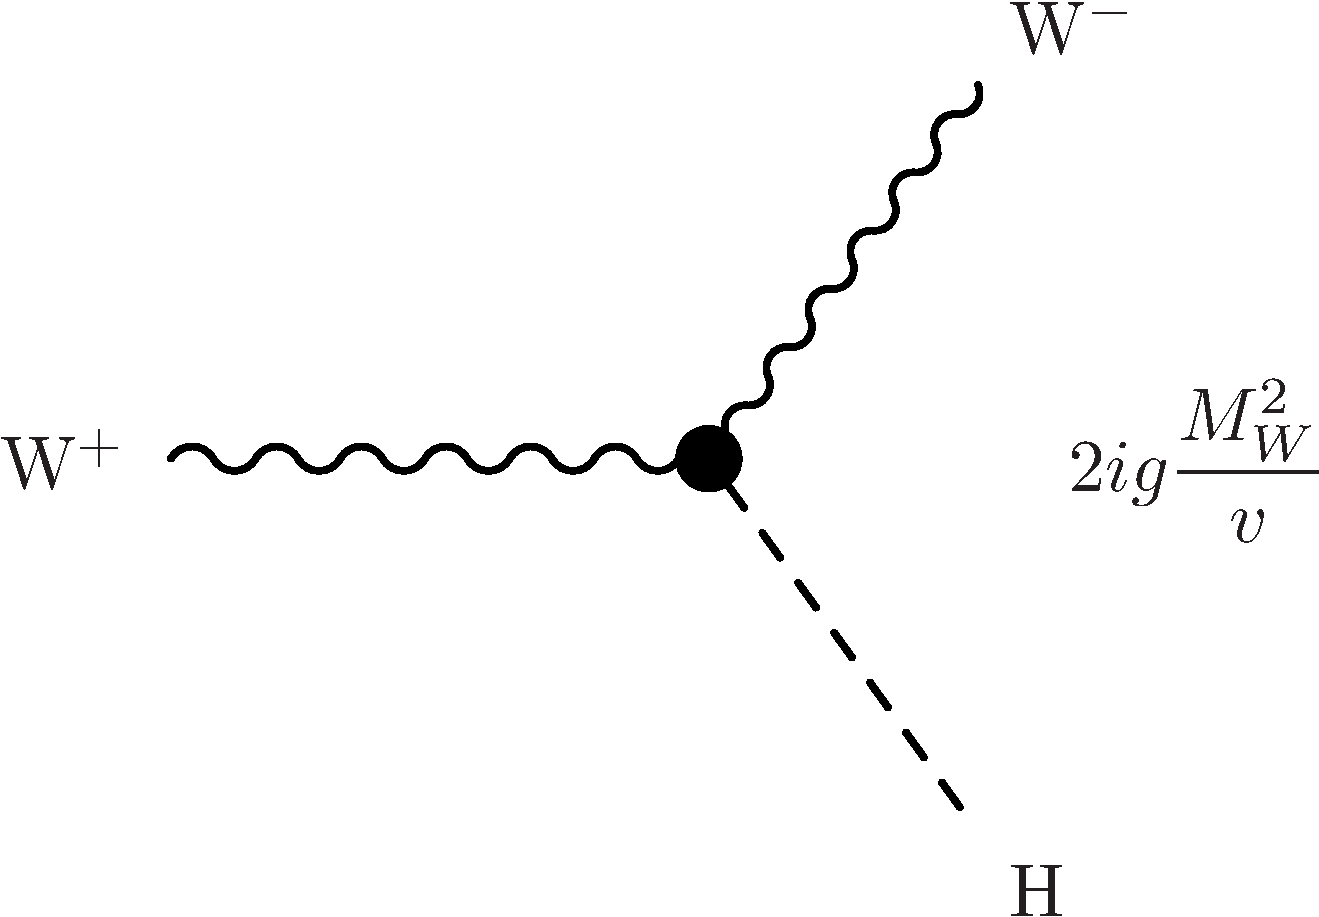
\includegraphics[width=0.3\textwidth]{\chtwo/Higgs_WWH_2.pdf}\hspace{0.4cm}
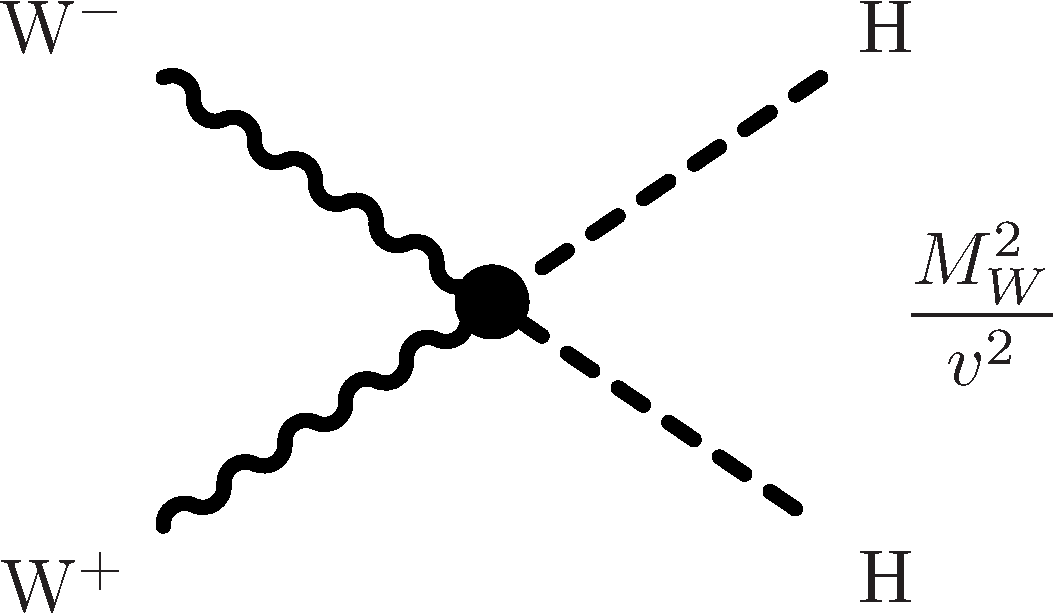
\includegraphics[width=0.3\textwidth]{\chtwo/Higgs_WWHH.pdf}\hspace{0.4cm}
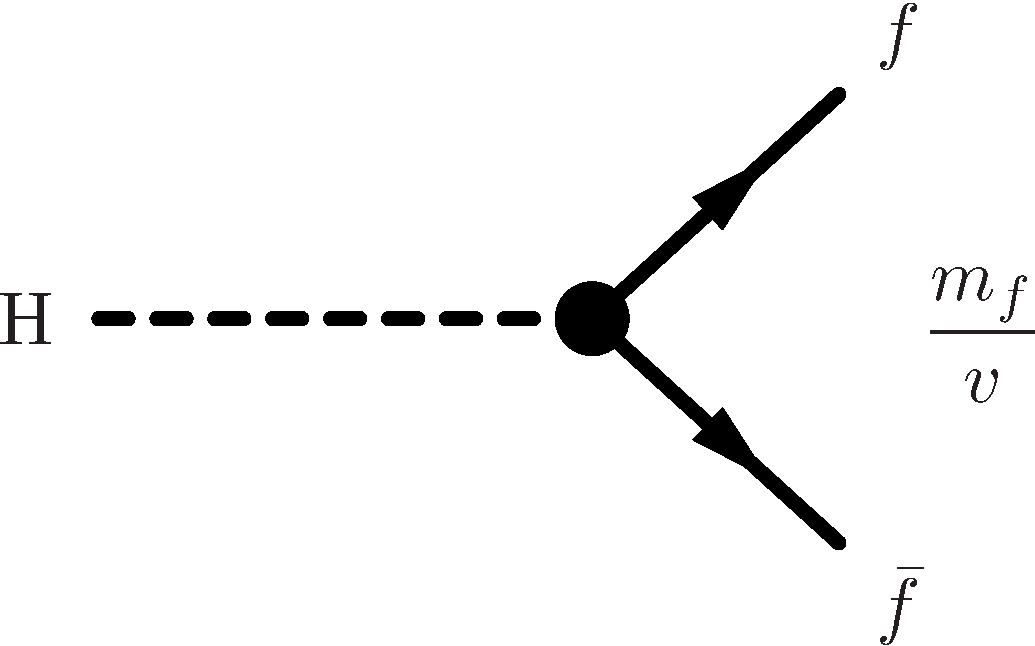
\includegraphics[width=0.3\textwidth]{\chtwo/Higgs_ffH.pdf}\\ \vspace{0.4cm}
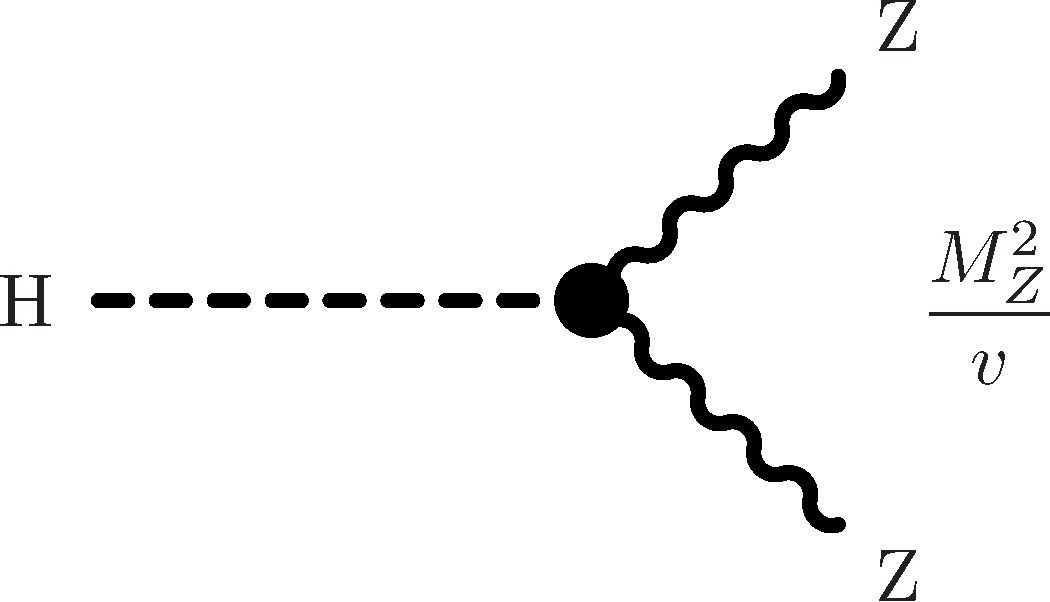
\includegraphics[width=0.3\textwidth]{\chtwo/Higgs_ZZH_2.pdf}\hspace{0.4cm}
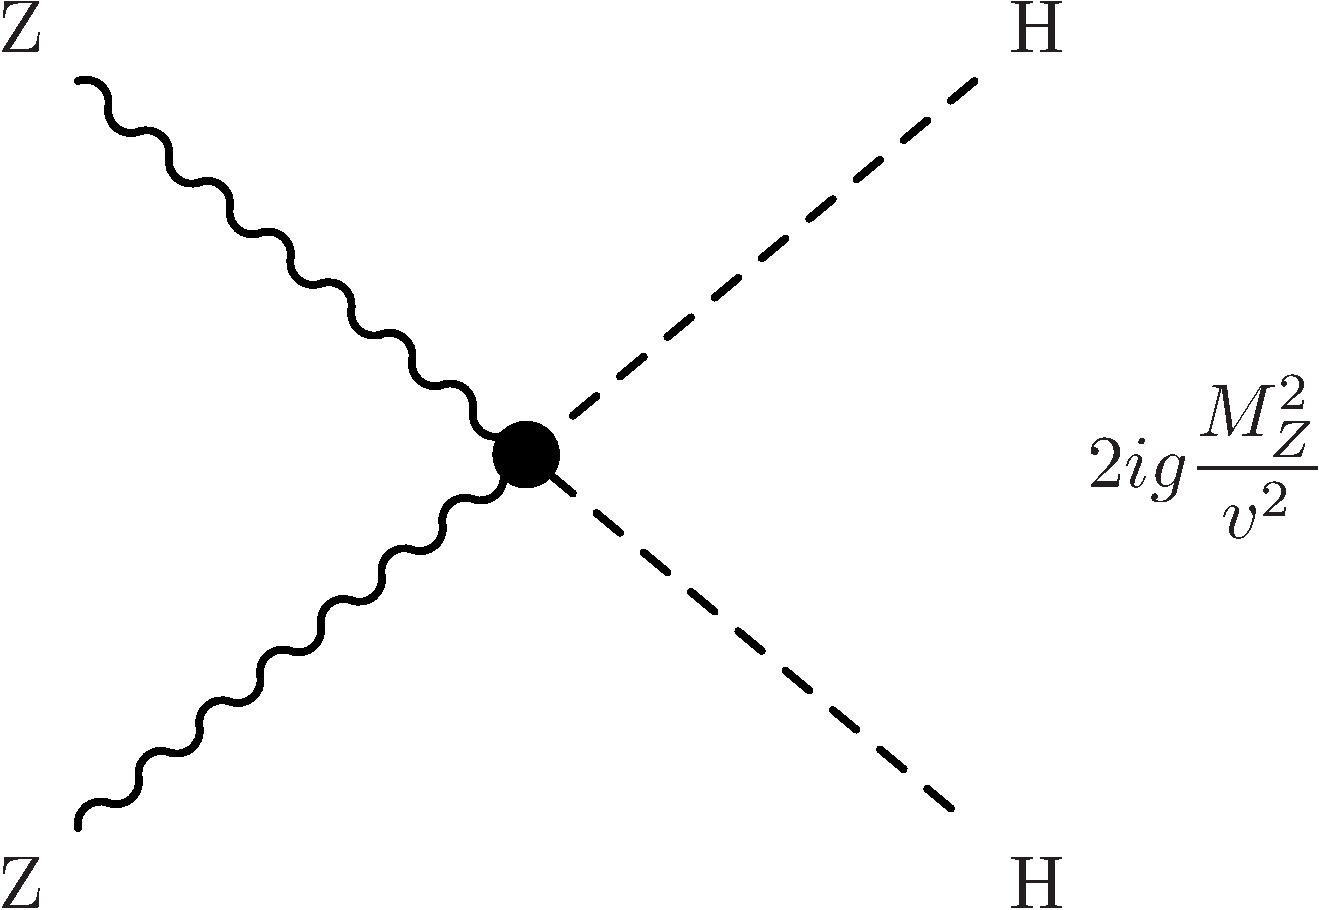
\includegraphics[width=0.3\textwidth]{\chtwo/Higgs_ZZHH.pdf}

\includegraphics[width=0.3\textwidth]{\chtwo/blank.png}\\ \vspace{0.4cm}
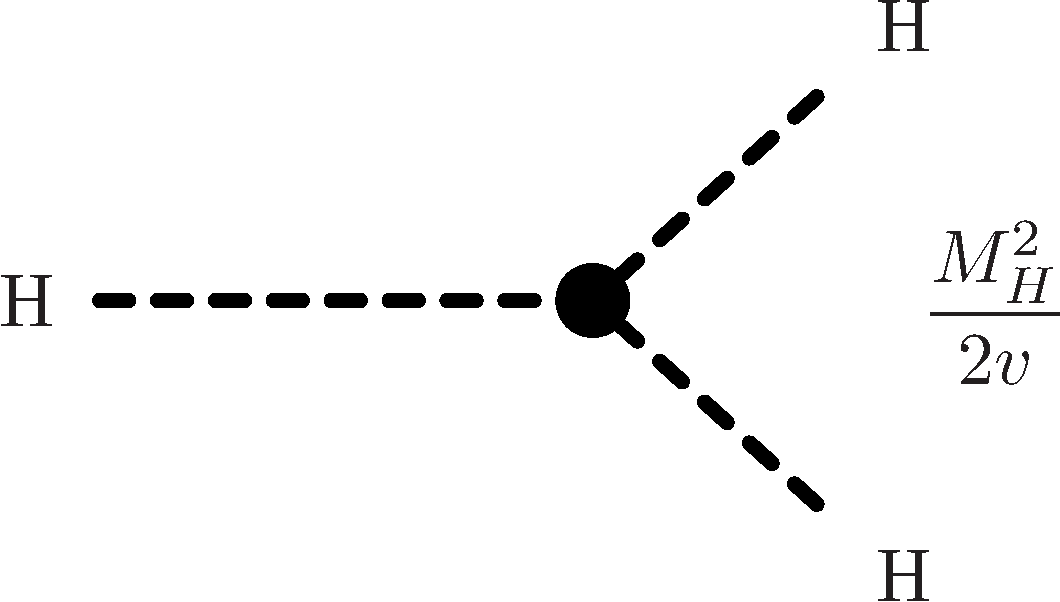
\includegraphics[width=0.3\textwidth]{\chtwo/Higgs_HHH.pdf}\hspace{0.4cm}
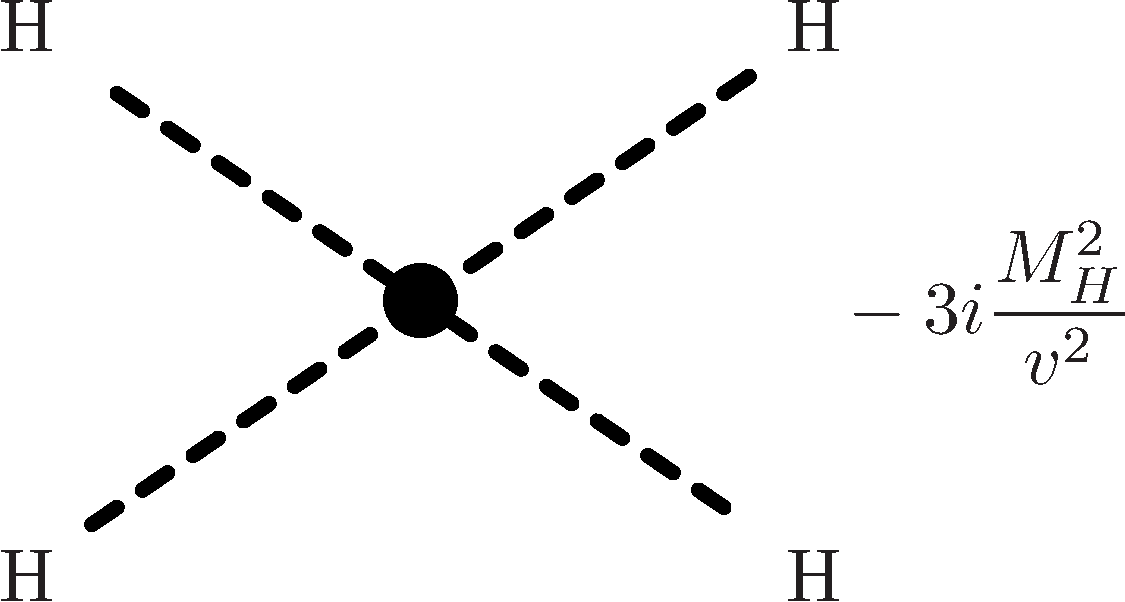
\includegraphics[width=0.3\textwidth]{\chtwo/Higgs_HHHH.pdf}

\includegraphics[width=0.3\textwidth]{\chtwo/blank.png}\\
\caption{Higgs interaction vertices in the standard model.}
\label{fig:HiggsSM}
\end{figure}

%Since, $\bar{\mathbf{f}}^\prime_L\mathbf{f}^\prime_L = \mathbf{f}_L\mathbf{f}_L$ and $\bar{\mathbf{f}}^\prime_R\mathbf{f}^\prime_R = \mathbf{f}_R\mathbf{f}_R$ ($f = u, d, \ell$),
%the form of the neutral-current part of the $\mathrm{SU(2)_L\times U(1)_Y}$ Lagrangian does not change when expressed in terms of mass eigenstates.
%Therefore, there are no flavor-changing neutral currents in the SM. %(GIM mechanism [4]).
%This is a consequence of treating all equal-charge fermions on the same footing.
%However, $\bar{\mathbf{u}}^\prime_L\mathbf{d}^\prime_L = \bar{\mathbf{u}}_L\mathbf{S}_u\mathbf{S}^\dag_d\mathbf{d}_L \equiv \bar{\mathbf{u}}_L\mathbf{V}\mathbf{d}_L$.
%In general, $\mathbf{S}_u \neq \mathbf{S}_d$; thus if one writes the weak eigenstates in terms of mass eigenstates, a $3\times3$ unitary mixing matrix $\mathbf{V}$, called the Cabibbo-Kobayashi-Maskawa (CKM) matrix\cite{CKM}, appears in the quark charged-current sector and couples any up-type quark with all down-type quarks:
%
%\begin{equation}\label{eqn:SM_e45}
%\begin{pmatrix}
%d^\prime \\ s^\prime \\ b^\prime
%\end{pmatrix}
%= \mathbf{V}
%\begin{pmatrix}
%d \\ s \\ b
%\end{pmatrix}_L
%=
%\begin{pmatrix}
%V_{ud} & V_{us} & V_{ub}\\
%V_{cd} & V_{cs} & V_{cb}\\
%V_{td} & V_{ts} & V_{tb}
%\end{pmatrix}
%\begin{pmatrix}
%d \\ s \\ b
%\end{pmatrix}_L
%\end{equation}
%
%The absolute values of its entries can be measured independently, but most precisely determined by a global fit that uses all available measurements.
%Requiring three generations of quarks and unitarity of the matrix yields the following absolute values~\cite{Olive:2016xmw,Hocker:2001xe,Charles2005}:
%
%\begin{equation}\label{eqn:SM_e46}
%\begin{pmatrix}
%0.97434^{+0.00011}_{-0.00012} & 0.22506 \pm 0.00050 & 0.00357 \pm 0.00015\\
%0.22492 \pm 0.00050                 & 0.97351 \pm 0.00013 & 0.0411 \pm 0.0013\\
%0.00875^{+0.00032}_{-0.00033} & 0.0403 \pm 0.0013    & 0.99915 \pm 0.00005
%\end{pmatrix}
%\end{equation}
%
%One observes large couplings close to 1 within the same generation (diagonal entries) whereas the off-diagonal entries are significantly smaller.
%With three quark generations, the unitarity requirement and taking into account that the quark phases cannot be measured the number of independent parameters of the matrix is reduced to four: three mixing angles between the quark generations and one complex phase that accounts for CP violation. Analogously, there exists a matrix describing the leptonic mixing, the Pontecorvo-Maki-Nakagawa-Sakata (PMNS) matrix~\cite{Ziro,PONTECORVO1968630}. It also contains four independent parameters if one assumes that neutrinos are not Majorana particles.

%%%%%%%%%%%%%%%%%%%%%%%%%%%%%%%%%%%%%%
\subsection{Observation of a particle compatible with the standard model Higgs boson}\label{subsec:HiggsLHC}
%%%%%%%%%%%%%%%%%%%%%%%%%%%%%%%%%%%%%%

The SM Higgs boson production cross sections at a proton-proton collider is shown in Fig.~\ref{fig:HiggsXS_a} as a function of the Higgs mass hypothesis and for the different leading production mechanisms.
In addition, in Fig.~\ref{fig:HiggsProd}, the corresponding Leading Order (LO) Feynman diagrams are shown.
Gluon fusion process ($gg \to \PH$) is the dominating Higgs production mechanism over the entire mass range accessible at the LHC.
In the vector boson fusion process  ($\mathrm{qq}^\prime \to \mathrm{qq}^\prime \PH$), which is about one order of magnitude weaker than gluon fusion, the Higgs boson is produced through a direct coupling with vector bosons (\PW or \PZ), which are irradiated by a pair of incoming quarks from the proton beams. 
The associated production with a \PW or \PZ boson ($\mathrm{q\bar{q}}^\prime \to \PW\PH$, $\qqbar \to \PZ\PH$) have a smaller cross section than the previous mechanisms but, the presence of the vector boson helps in reconstructing the events reducing the contamination from other SM processes.
The associated production with \ttbar pairs (qq, $gg \to \ttbar\PH$) has the smallest cross section, however, it allows for a direct access to the Higgs coupling to top quarks, representing thus an important process.
Depending on the Higgs boson mass hypothesis, different decay channels (Fig.~\ref{fig:HiggsXS_b}) can be exploited to detect it.
The Higgs boson does not couple to photons and gluons at LO, but such processes can arise via fermion or vector boson loops, giving a sizable contribution in the low mass region.\\

\begin{figure}[!htb]
\centering
\subfigure[]{\label{fig:HiggsXS_a}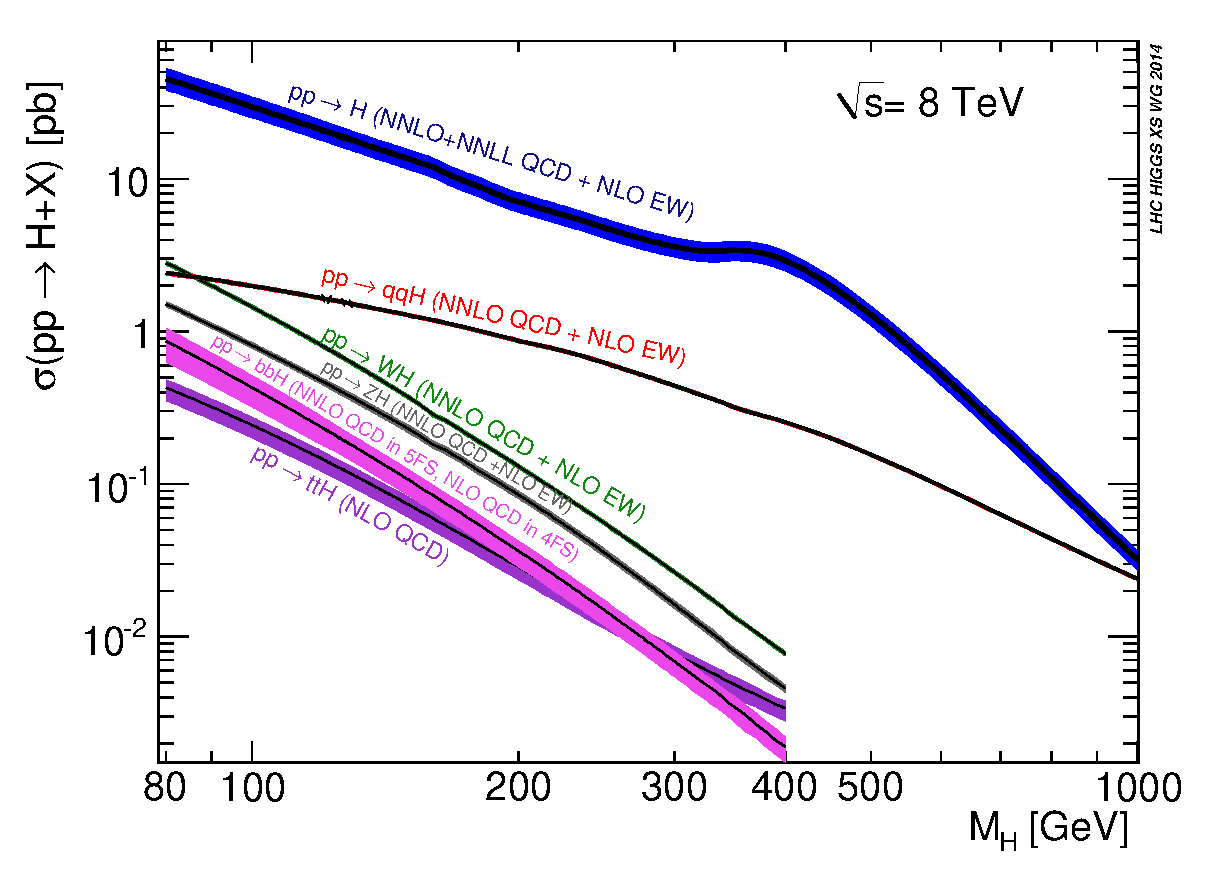
\includegraphics[width=0.56\textwidth]{\chtwo/XS_8TeV.eps}}
\subfigure[]{\label{fig:HiggsXS_b}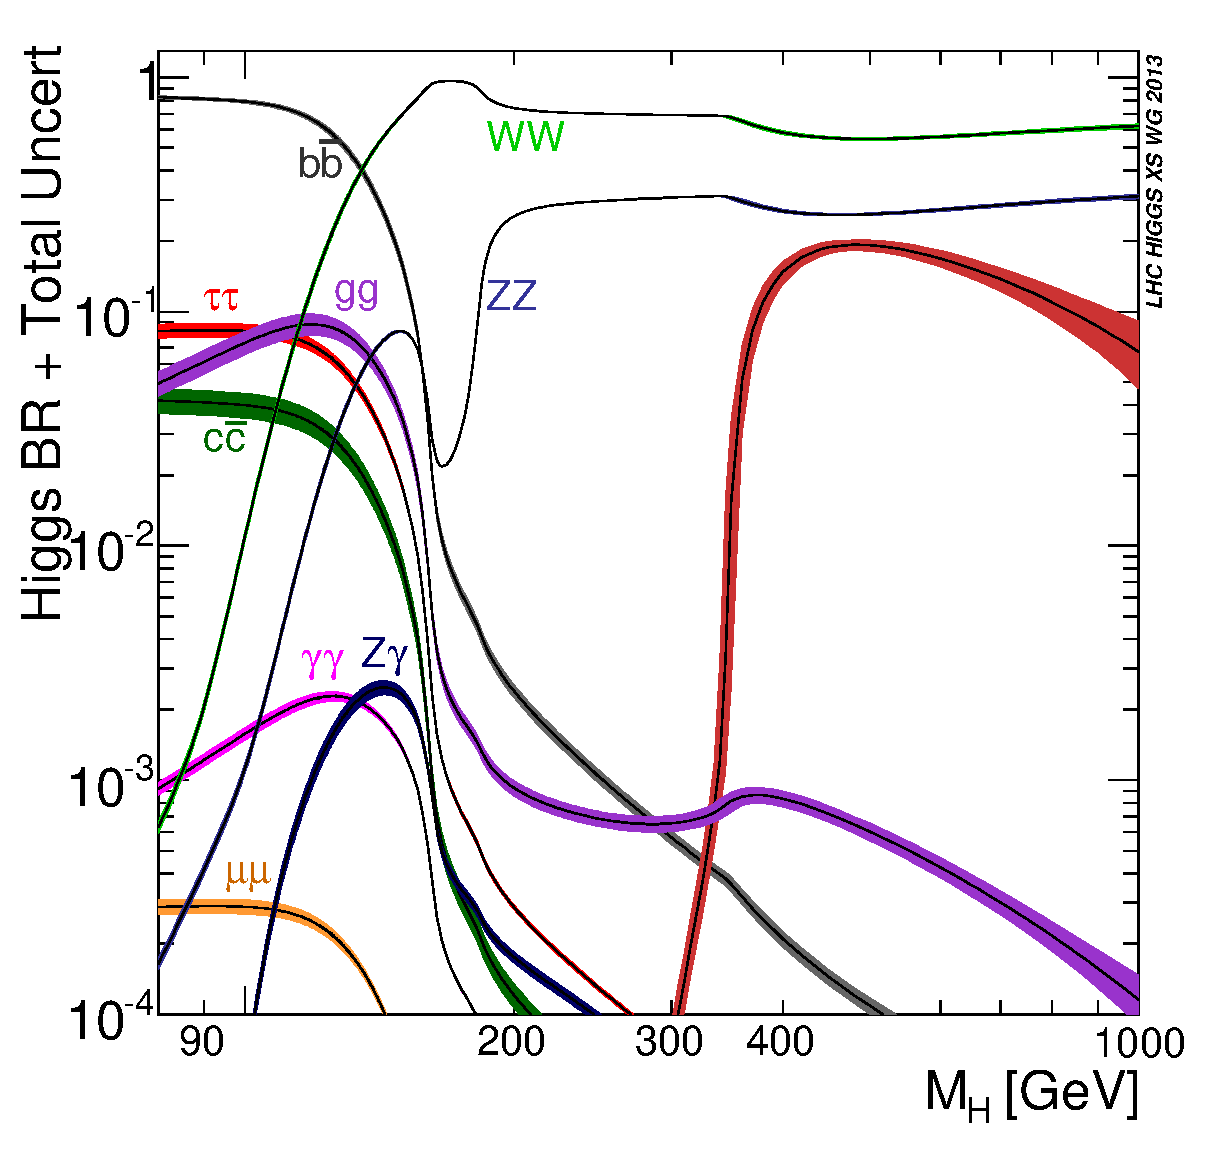
\includegraphics[width=0.42\textwidth]{\chtwo/Higgs_BR.eps}}
\caption{(a) The SM Higgs production cross-sections at $\sqrt{s} = 8\TeV$ for the different production mechanisms~\cite{Dittmaier:2011ti}. (b) Decay branching ratios of the SM Higgs boson in the different channels as a function of the mass hypothesis~\cite{Dittmaier:2011ti}.}
\label{fig:HiggsXS}
\end{figure}

\begin{figure}[!htb]
\centering
\subfigure[]{\label{fig:HiggsProd_a}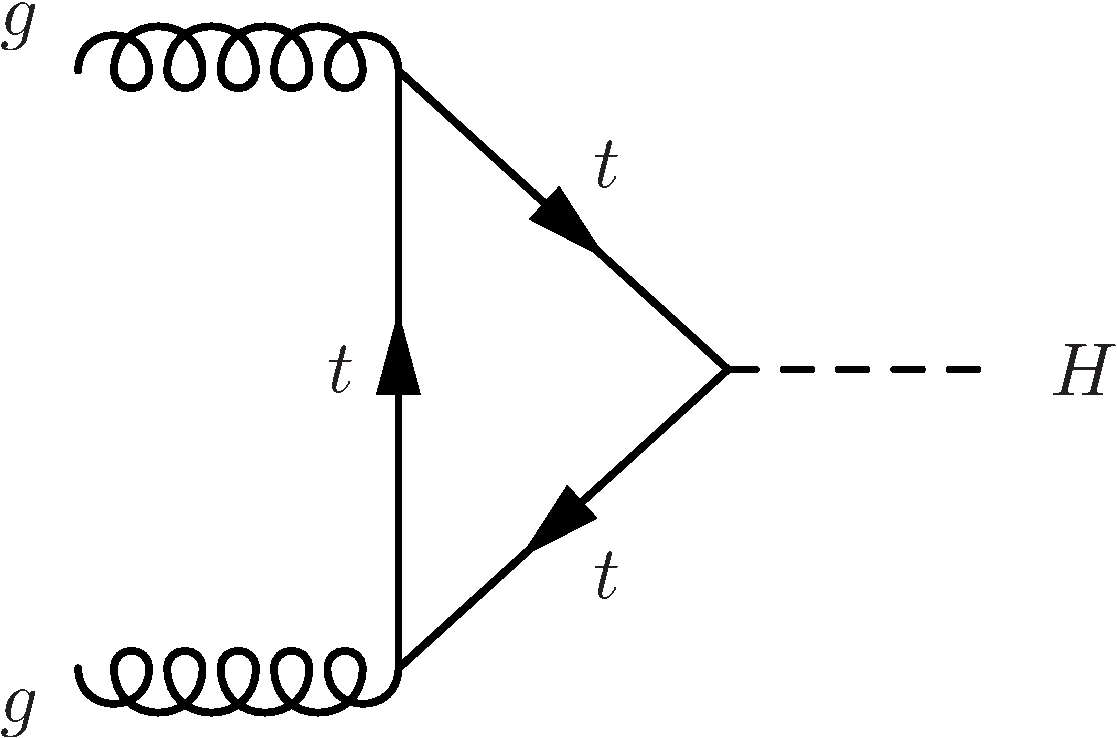
\includegraphics[width=0.23\textwidth]{\chtwo/Higgs_GF.pdf}}
\subfigure[]{\label{fig:HiggsProd_b}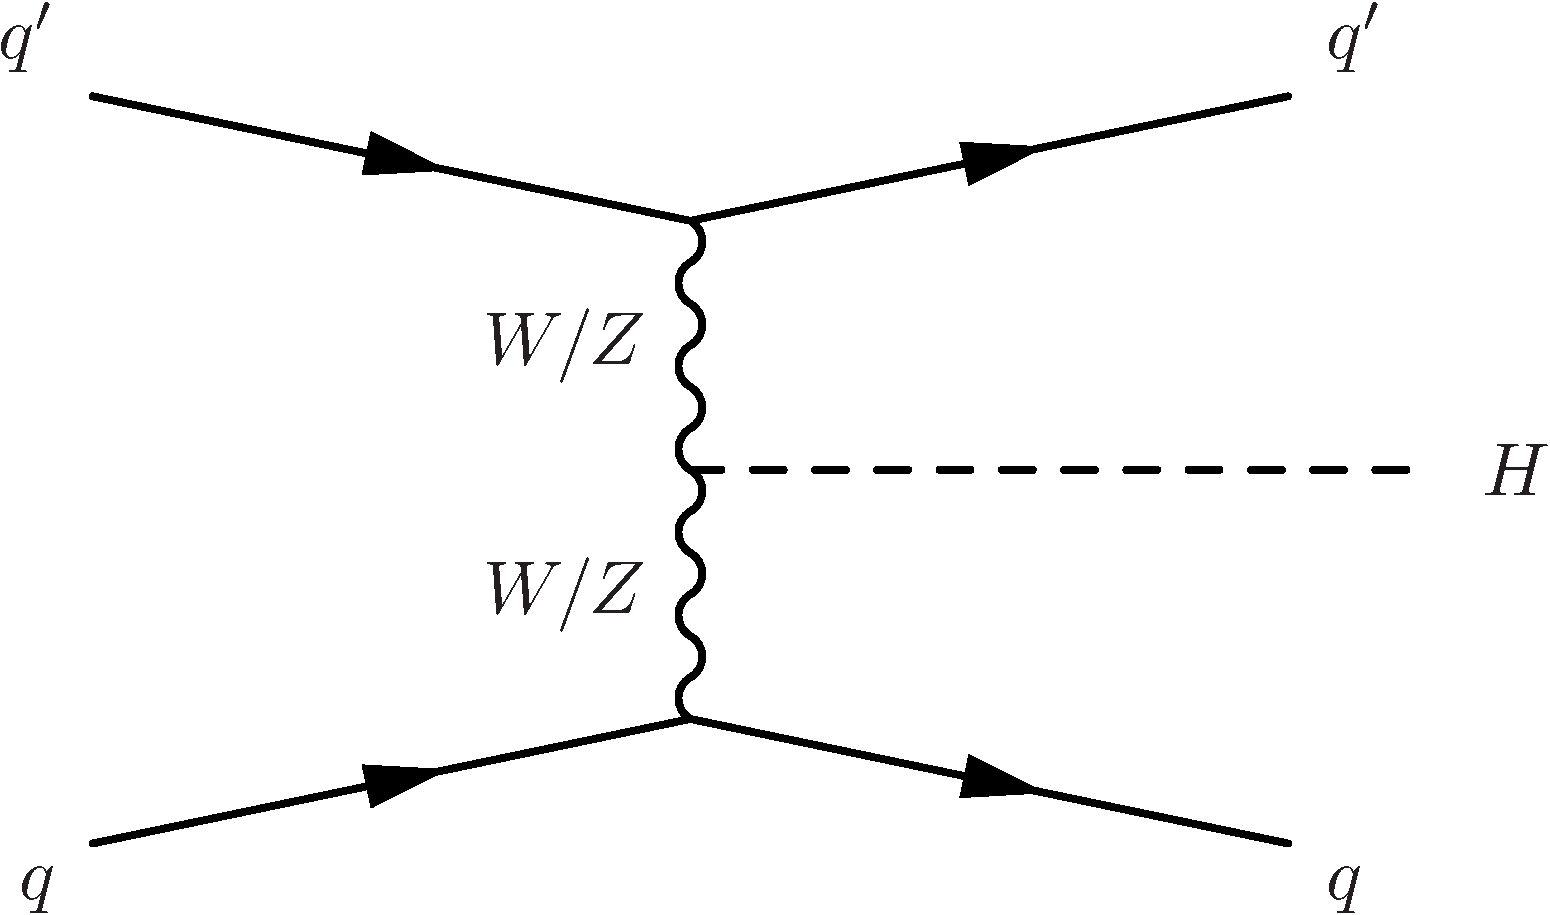
\includegraphics[width=0.23\textwidth]{\chtwo/Higgs_VBF.pdf}}
\subfigure[]{\label{fig:HiggsProd_c}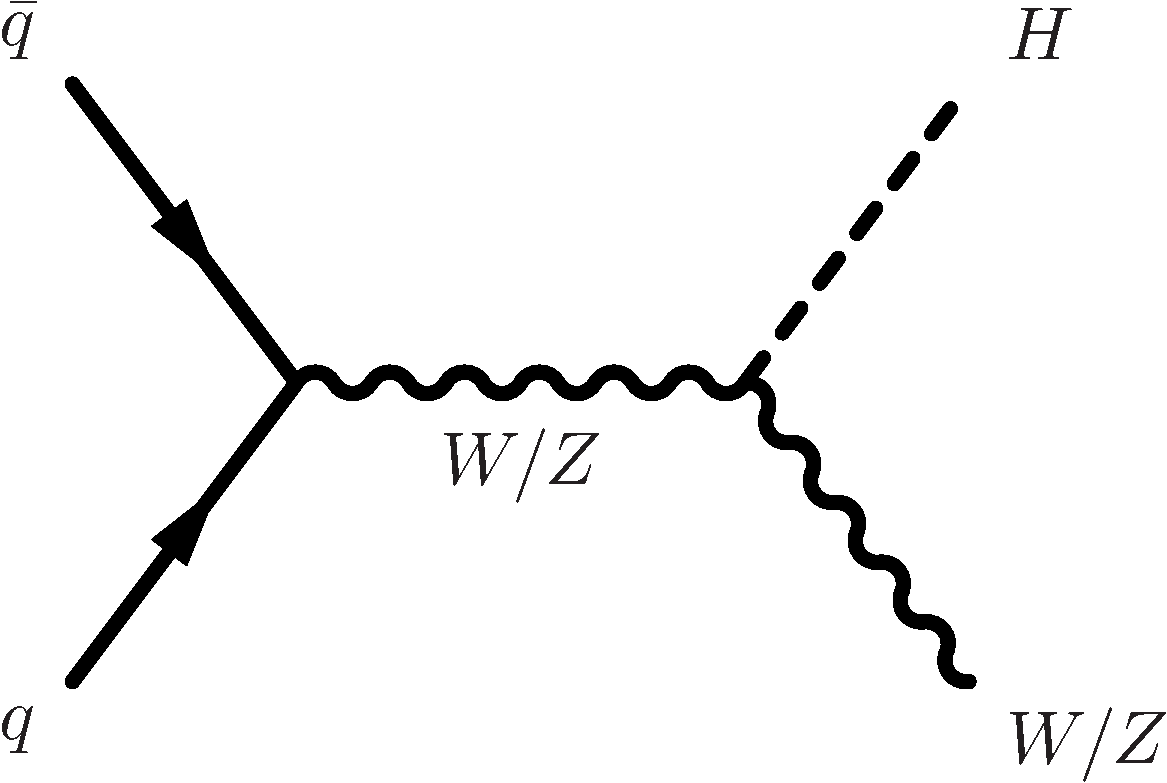
\includegraphics[width=0.23\textwidth]{\chtwo/Higgs_VH.pdf}}
\subfigure[]{\label{fig:HiggsProd_d}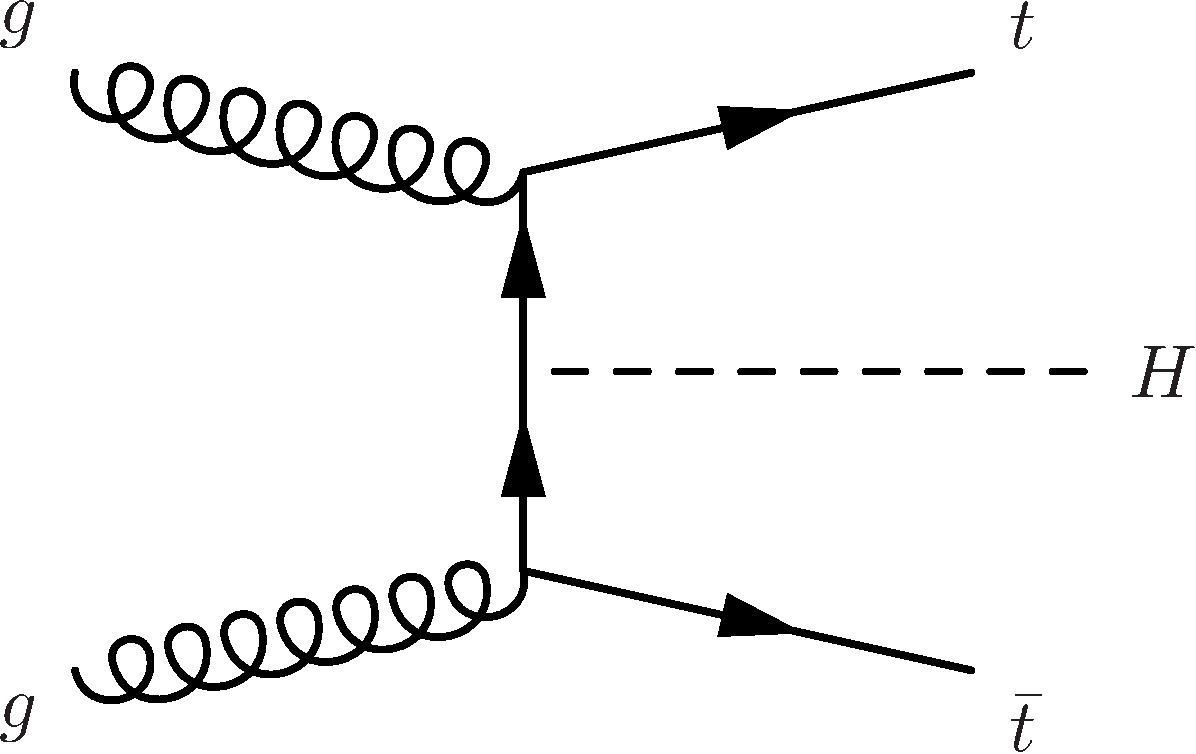
\includegraphics[width=0.23\textwidth]{\chtwo/Higgs_ttH.pdf}}
\caption{Leading order Feynman diagrams for the most important production processes of the SM Higgs boson: (a) gluon fusion, (b) vector boson fusion, (c) Higgs-strahlung and (d) \ttbar associated production.}
\label{fig:HiggsProd}
\end{figure}

The search for the massive Higgs boson has been long and tedious. 
However, in Summer 2012, the ATLAS and the CMS collaborations announced the observation of a new particle in data taken in 2011 and 2012~\cite{Chatrchyan:2013lba,Aad:2012tfa}.
A combination of the measurements targeting its decay into fermions ($\bbbar$, $\tau\tau$) or vector bosons ($\PZ\PZ^*$, $\PW\PW^*$, $\gamma\gamma$) and all the different production modes, led to an excess of events above the expected background around a mass of 125\GeV.
The CMS result yields a local significance of $5.0\sigma$ with a global significance of $4.6\sigma$ in the Higgs mass search range of $115 < m_\PH < 130\GeV$ (Fig.~\ref{fig:HiggsPvalue_a}).
For ATLAS, the local significance is found to be $5.9\sigma$ with a global significance of $5.1\sigma$ in the range $100 < m_\PH < 600\GeV$ (Fig.~\ref{fig:HiggsPvalue_b}).
A simultaneous fit to the reconstructed invariant mass peaks in the two channels with the highest mass resolution, $\PH \to \PZ\PZ^* \to 4\ell$ and $\PH \to \gamma\gamma$ , and for the two experiments has been performed.
The resulting combined measured mass of the Higgs boson is $m_\PH = 125.09 \pm 0.21 \mbox{(stat.)} \pm 0.11 \mbox{(syst.)} \GeV$ (Fig.~\ref{fig:HiggsMass})~\cite{Aad:2015zhl}.
Subsequent studies on production and decay rates~\cite{Khachatryan:2016vau} and spin-parity~\cite{Aad:2015mxa,Chatrchyan:2012jja,Khachatryan:2014kca} of the new boson showed that its properties are compatible with those expected for the SM Higgs boson. 

  \begin{figure}[!htb]
  \centering
  \subfigure[]{\label{fig:HiggsPvalue_a}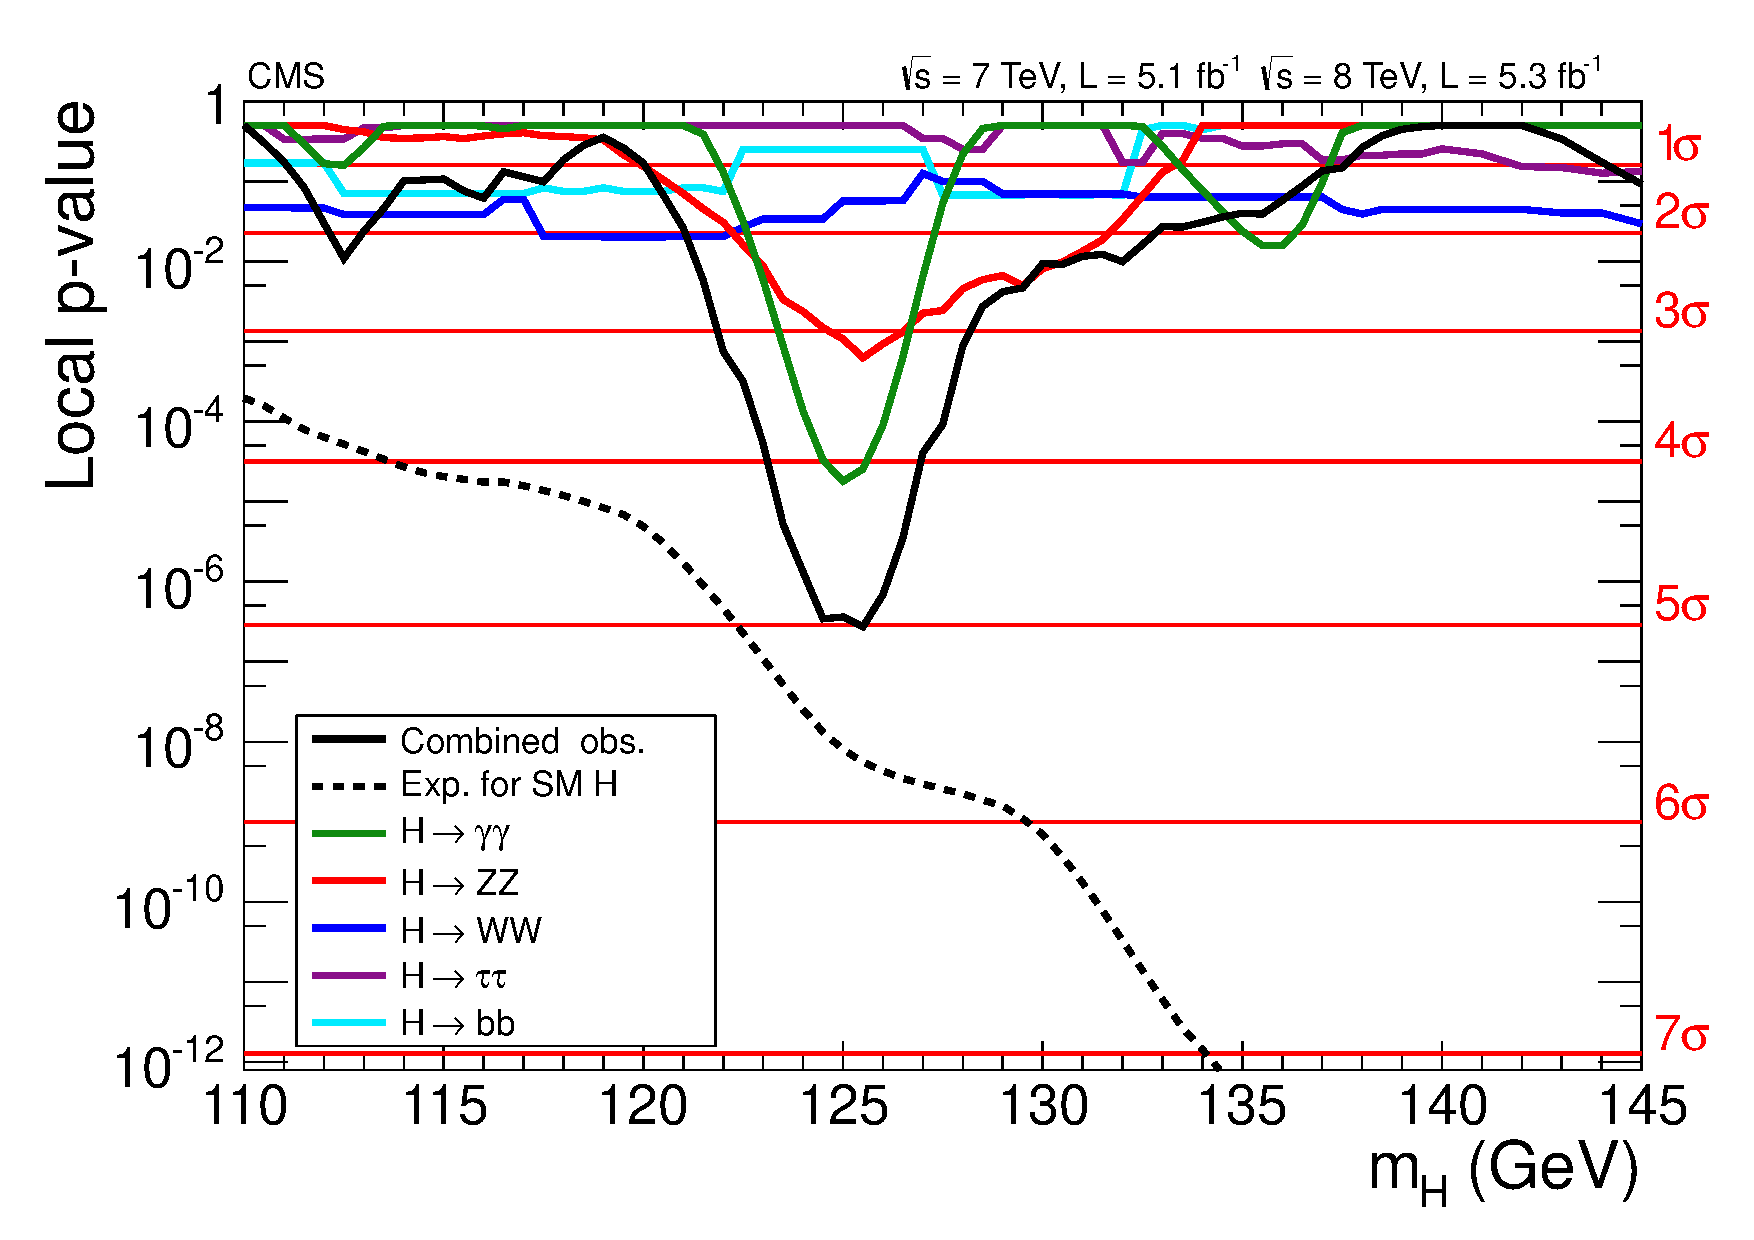
\includegraphics[width=0.45\textwidth]{\chtwo/rect_pvala_all_bydecay_smallGGScale_wideX.pdf}}
  \subfigure[]{\label{fig:HiggsPvalue_b}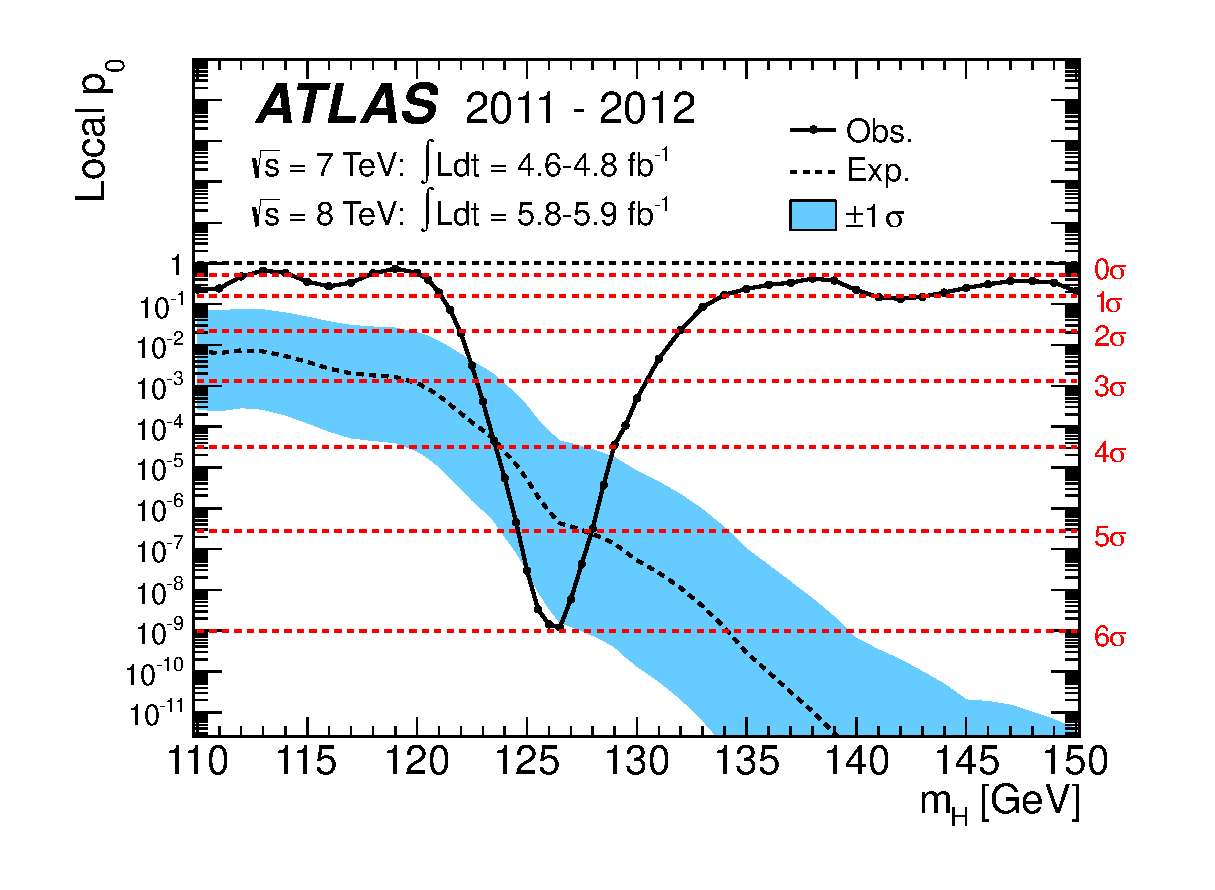
\includegraphics[width=0.45\textwidth]{\chtwo/HiggsDiscovery_ATLAS_pvalue.eps}}
  \caption{The observed (solid) local p-value as a function of the Higgs boson mass $m_\PH$ for (a) the CMS and (b) ATLAS experiments. In (a) the results for each individual channel are also shown. 
  The dashed curve shows the expected local p-value under the hypothesis of a SM Higgs boson signal at that mass.
  The horizontal red lines indicate the p-values corresponding to significances of 1 to 6$\sigma$.}
  \label{fig:HiggsPvalue}
\end{figure} 

  \begin{figure}[!htb]
  \centering
  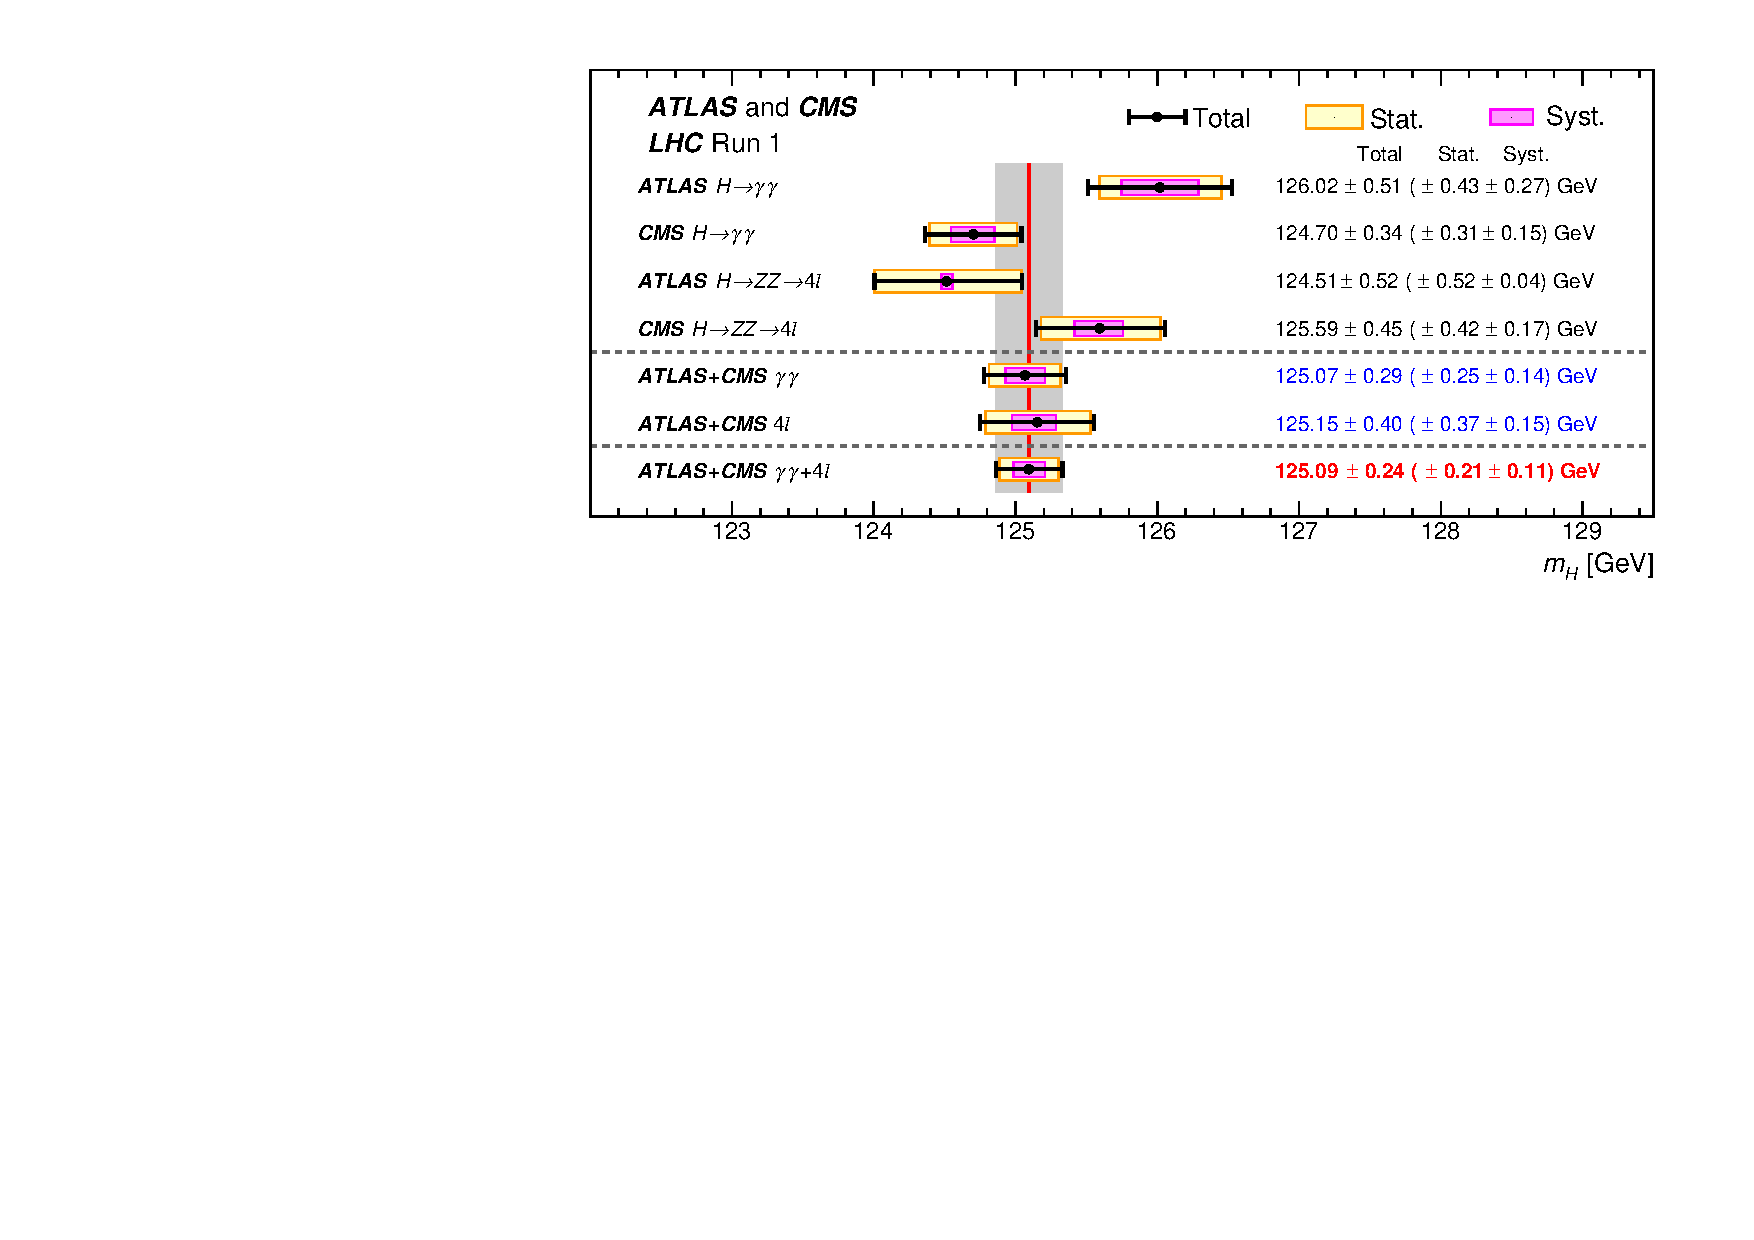
\includegraphics[width=0.7\textwidth]{\chtwo/LHC_combined_obs_unblind_summary_a1_final.pdf}
  \caption{Summary of Higgs boson mass measurements from the individual analyses of ATLAS and CMS and from their combination.
  The magenta and yellow bands correspond to the the systematic and statistical uncertainties, respectively. The total uncertainties are also indicated as black error bars.
  The red vertical line and corresponding gray shaded column indicate the central value and the total uncertainty of the combined measurement, respectively~\cite{Aad:2015zhl}.}
  \label{fig:HiggsMass}
\end{figure} 

Finally, the Higgs boson couplings to SM particles are investigated simultaneously in different production and decay processes, including the possibility of the Higgs boson to be coupled to BSM particles~\cite{Khachatryan:2016vau}.
To test possible deviations from the SM predictions, the coupling modifiers, $k^2_j = \sigma_j/\sigma^\mathrm{SM}_j$ and $k^2_j = \Gamma_j/\Gamma^\mathrm{SM}_j$, for production and decay rates, are introduced. 
However, to directly measure the individual coupling modifiers, an assumption about the Higgs boson width $\Gamma_\PH$ is necessary. Thus, another modifier is introduced and defined as $k_\PH = \sum_j \mathcal{B}^\mathrm{SM}_jk^2_j$, where $\mathcal{B}^\mathrm{SM}_j$ are the branching fractions for the Higgs boson decay to the final state $f$ as predicted by the SM. In the case where the SM decays of the Higgs boson are the only ones allowed,
the relation $k^2_\PH = \Gamma_\PH/\Gamma^\mathrm{SM}_\PH$ holds. If instead deviations from the SM are introduced in the decays, the width can be expressed as:

\begin{equation}\label{eqn:SM_e45}
\Gamma_\PH = \frac{k^2_\PH\Gamma^\mathrm{SM}_\PH}{1 - B_\mathrm{BSM}},
\end{equation}

\noindent where $B_\mathrm{BSM}$ indicates the total branching fraction into BSM decays.
The two possible scenarios are considered: the first leaves $B_\mathrm{BSM}$ free, provided that $B_\mathrm{BSM} \geq 0$, whereas the second assumes $B_\mathrm{BSM} = 0$. 
The parameters of interest in the fits to data are thus the seven independent coupling modifiers, $k_\PZ$, $k_\PW$, $k_\mathrm{t}$, $k_\tau$, $k_\mathrm{b}$, $k_g$, and $k_\gamma$, 
one for each SM particle involved in the production processes and decay modes studied, plus $B_\mathrm{BSM}$ in the case of the first scenario.
The results of the two fits are shown in Fig.~\ref{fig:HiggsCoupl}.
The overall branching fraction of the Higgs boson into BSM decays is determined to be less than 34\% at 95\% CL.
This constraint applies to invisible decays into BSM particles, decays into BSM particles that are not detected as such, and modifications of the decays into SM particles that are not directly measured by the experiments.

  \begin{figure}[!htb]
  \centering
  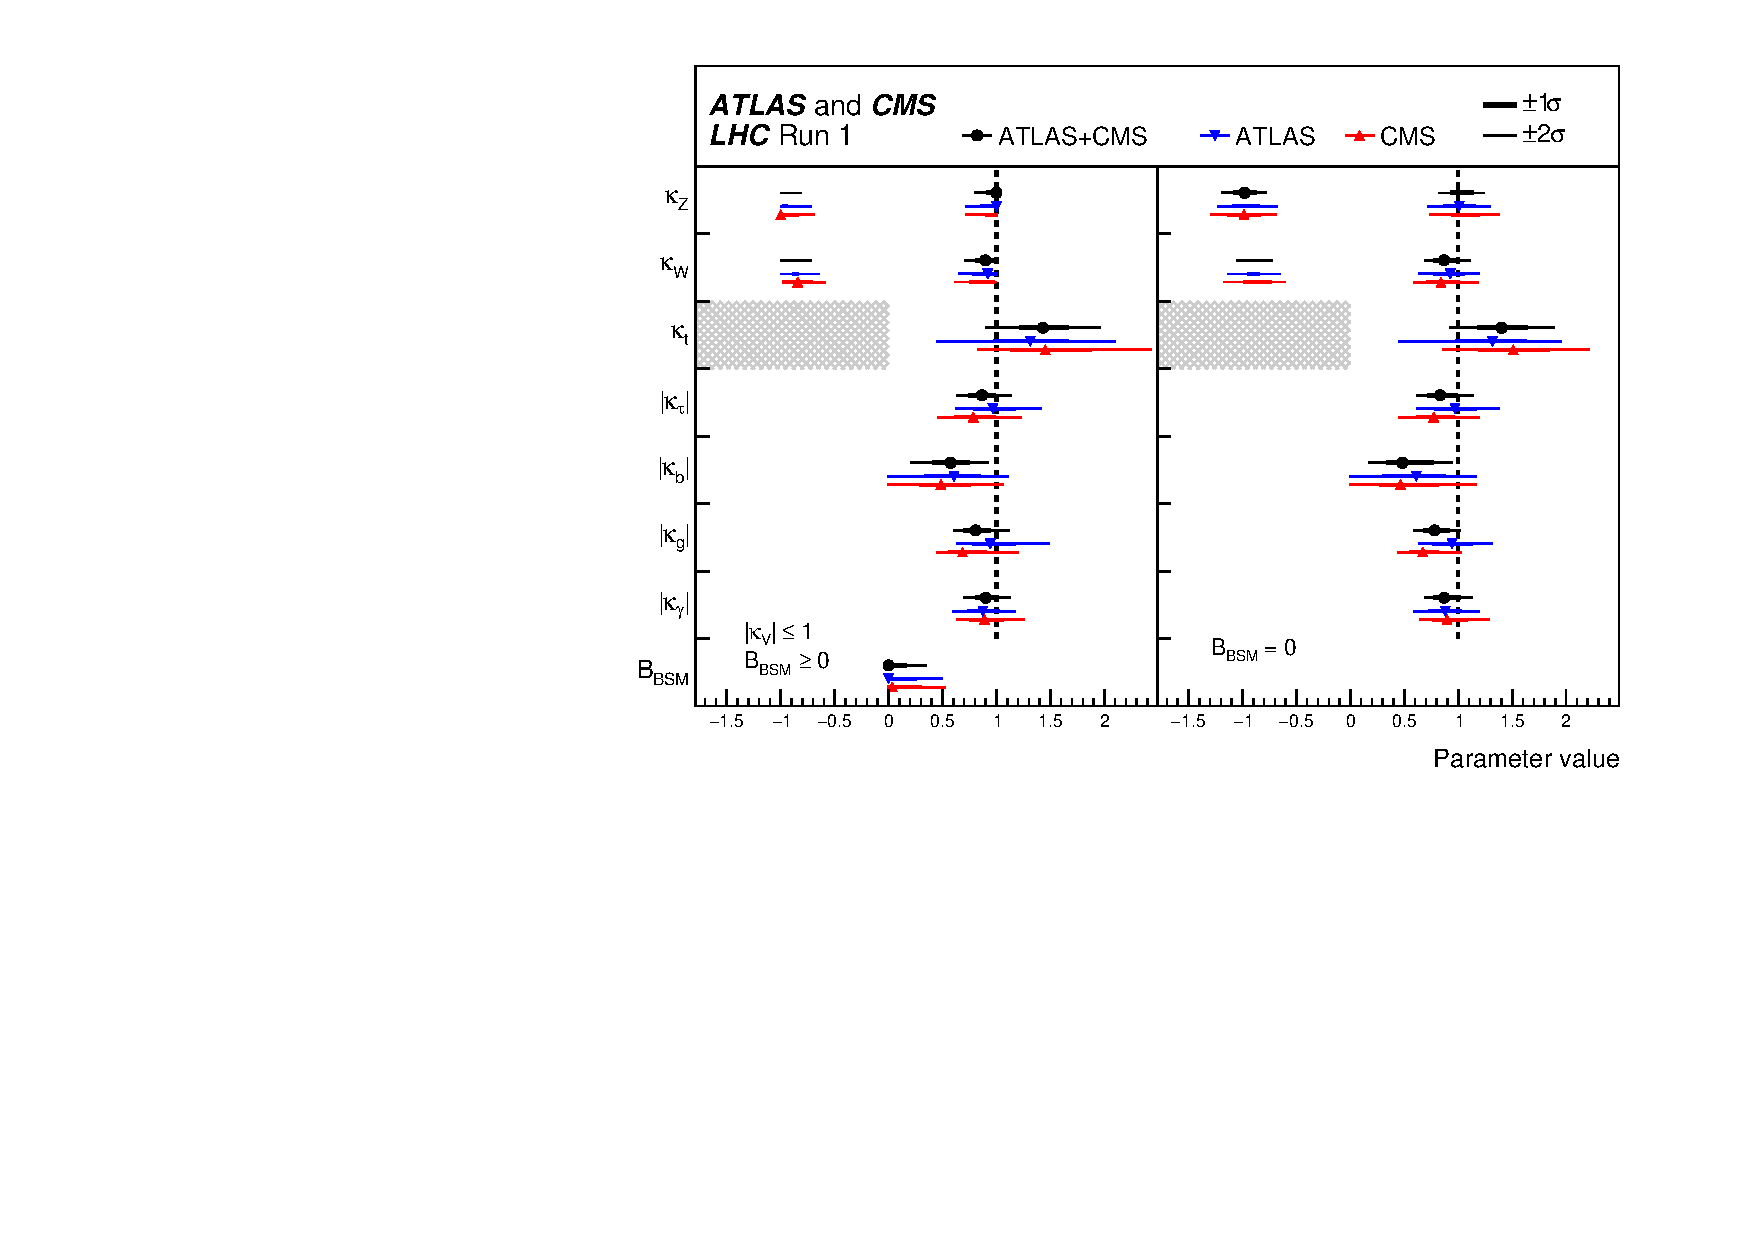
\includegraphics[width=0.7\textwidth]{\chtwo/plot_K2_K2_BRinv_per_exp_merged.pdf}
  \caption{Fit results for two parameterizations: the first one assumes that $B_\mathrm{BSM} \geq 0$, and the second one assumes that there are no additional BSM contributions to the Higgs boson width ($B_\mathrm{BSM} = 0$). The measured results for the combination of ATLAS and CMS are reported together with their uncertainties, as well as the individual results from each experiment~\cite{Aad:2015zhl}.}
  \label{fig:HiggsCoupl}
\end{figure} 

%%%%%%%%%%%%%%%%%%%%%%%%%%%%%%%%%%%%%%%%%
\subsection{Quantum chromodynamics}\label{subsec:QCD}
%%%%%%%%%%%%%%%%%%%%%%%%%%%%%%%%%%%%%%%%%

Quantum Chromodynamics (QCD) is the gauge theory of strong interactions, describing the dynamics of colored quarks and gluons.
The QCD represents the $SU(3)_C$ component of the standard model, where $C$ denotes the color.
After applying the principle of gauge invariance to the free Lagrangian for the quark fields holding color $\alpha$ that runs from 1 to 3 (usually identified with red, green, blue), and flavor $q$, one obtains the following expression for the final gauge invariant QCD Lagrangian

\begin{equation}\label{eqn:SM_e46}
\mathcal{L}_\mathrm{QCD} = \sum_{q} \bar{\psi}_{q,\alpha} (i\gamma^\mu\partial_\mu\delta_{\alpha\beta} - g_s\gamma^\mu t^a_{\alpha\beta}\mathcal{A}^a_\mu - m_q\delta_{\alpha\beta})\psi_{q,b} - \frac{1}{4}G^a_{\mu\nu}G^{\mu\nu}_a.
\end{equation}

In the equation above, the quark fields are represented by the spinors $\psi$. The fields $\mathcal{A}^a_\mu$ corresponds to the eight gluon fields, since $C$ runs from 1 to $N^2_C - 1 = 8$.
Each gluon carries one unit of color and one unit of anticolor.
The eight $3\times3$ matrices $t^a_{\alpha\beta}$ are the $SU(3)_C$ generators and rotate the quark color in the $SU(3)_C$ space in a quark-gluon interaction.
The field tensor is

\begin{equation}\label{eqn:SM_e47}
G^a_{\mu\nu} = \partial_\mu\mathcal{A}^a_\nu - \partial_\nu\mathcal{A}^a_\mu - g_s f_{abc}\mathcal{A}^b_\mu\mathcal{A}^c_\nu,
\end{equation}

\noindent where $f_{abc}$ are the structure constants of the $SU(3)$ group.
As $[t^a,t^b] = if_{abc}t^c$ the group is non-Abelian. Owing this property, $G^a_{\mu\nu}G^{\mu\nu}_a$ term generates the cubic and quartic gluon self-interactions.
The fundamental parameters of QCD are the \textit{strong coupling constant} $g_s$, often written in terms of $\alpha_s = g_s^2/4\pi$, and the quark masses $m_q$.
All interactions appearing in Eq.~\ref{eqn:SM_e45} have strength given by $g_s$ (Fig.~\ref{fig:QCDVtx}).\\

\begin{figure}[!htb]
\centering
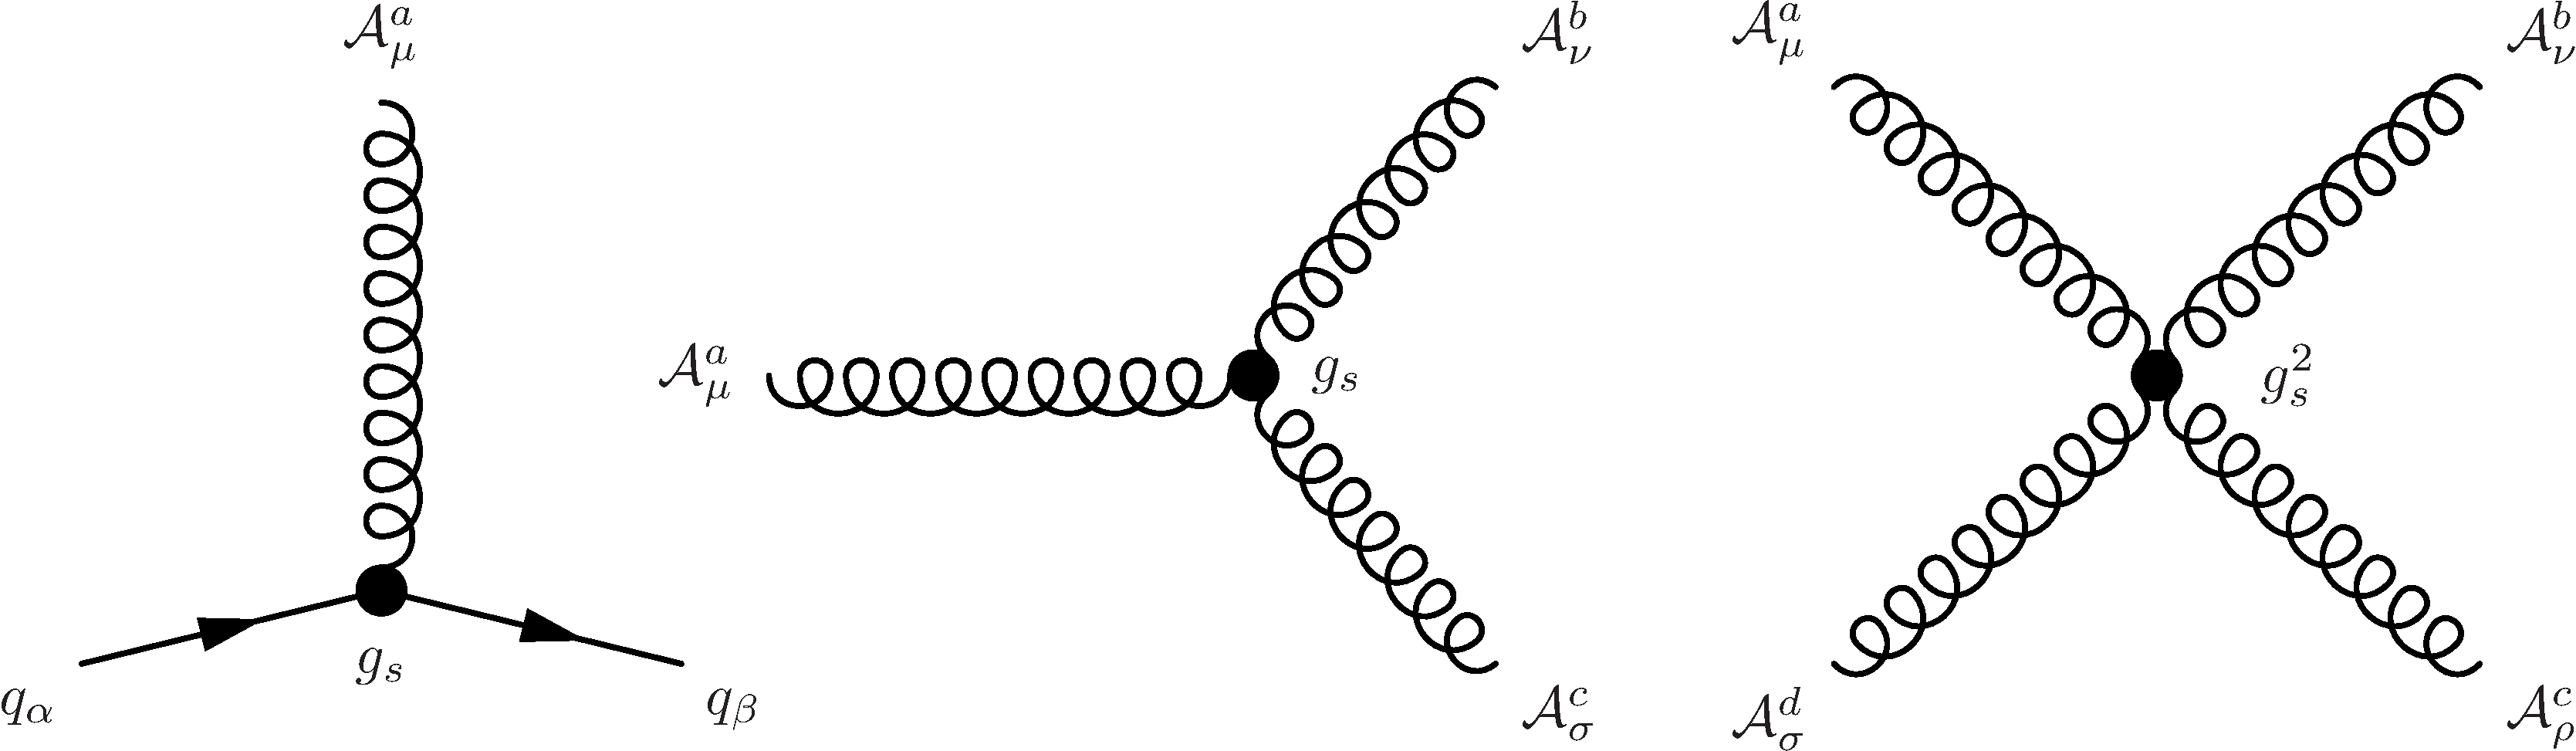
\includegraphics[width=0.9\textwidth]{\chtwo/QCD_vtx.pdf}
\caption{Interaction vertices of the QCD Lagrangian.}
\label{fig:QCDVtx}
\end{figure}

The QCD has the property of \textit{asymptotic freedom}, i.e. the coupling becomes weak at high energies or short distances, and for energies approaching zero or for very large distances, it tends to infinity.
As a consequence, the further away a quark is pulled from another one, the stronger the force gets, such that quarks cannot exist as free particles.
Because of this phenomenon, referred to as \textit{confinement}, quarks form bound color-singlet states called hadrons, consisting of either a quark and an antiquark (mesons) or three quarks or antiquarks (baryons).
%As a consequence, only in very high momentum transfer interactions, quarks can be regarded as free particles, whereas at low energy or large distance, the interaction becomes strongly coupled leading to \textit{confinement} of quarks %and gluons. Instead, they form bound color-singlet states called hadrons, consisting of either a quark and an antiquark (mesons) or three quarks or antiquarks (baryons).
%In this process, after a quark production, at very short distances, the quantum nature of QCD predicts the generation of virtual quark-antiquark (or gluons) pairs, which couple together through color strings forming observable un-%colored baryons and mesons.
In the regime of very high momentum transfer interactions, the perturbation theory is a very satisfactory description of QCD physics observables, giving precise predictions about what can be tested in collider experiments. This approach is called perturbative-QCD, or pQCD. In this framework, QCD predictions are calculated using the formalism of the Feynman rules which are derived from the $\mathcal{L}_\mathrm{QCD}$.
The transition amplitudes for a given process from a set of initial state particles to a set of final state particles are computed by sorting the diagrams by the factors of the coupling constants and calculating them up to a certain order.
However, higher order diagrams generally contain loops which contribute and lead to divergencies.
In order to obtain finite predictions for the cross sections, a renormalization of the theory is performed, resulting in a cancellation of the divergent terms.
%The divergencies are absorbed into a redefinition of the color charge. As a consequence of this, $\alpha_s$ is a running coupling constant as a function of a renormalization scale $\mu_R$, and is given by
The predictions for observables are then expressed in terms of the renormalized coupling $\alpha_s(\mu^2_R)$, a function of the renormalisation scale $\mu_R$. 
The coupling satisfies the renormalisation group equation:

\begin{equation}\label{eqn:SM_e48}
\mu^2_R\frac{\mathrm{d}\alpha_s}{\mathrm{d}\mu^2_R} = \beta(\alpha_s) = - (b_0\alpha^2_s + b_1\alpha^3_s + b_2\alpha^4_s + \dotsc)
\end{equation}

\noindent where the $b_i$ are the $i$-loop coefficients of the $\beta$ function.
They depend on the number of quark flavors $n_f$, and for sixteen or less flavors the strong coupling gets smaller for processes that involve large momentum transfer, leading to the asymptotic freedom.
Choosing $\mu_R$ close to the typical scale of the process of interest $Q^2$, the $\alpha_s(\mu_R)$ represents the effective strength of the strong interaction between particles under study.
Neglecting all the $b_i$ coefficients but $b_0$, an exact leading order expression for the running coupling $\alpha_s$ can be obtained

\begin{equation}\label{eqn:SM_e49}
\alpha_s(\mu^2_R) = \frac{1}{b_0\log \left( \frac{\mu^2_R}{\Lambda^2_\mathrm{QCD}} \right) } = \frac{12\pi}{(33-2n_f)\log \left( \frac{\mu^2_R}{\Lambda^2_\mathrm{QCD}} \right) }
\end{equation}

\noindent where $\Lambda_\mathrm{QCD}$ is the perturbative cut-off over the renormalization's integrals, and is not predicted by the theory.
The meaning of this cut-off is the validity of the perturbative regime approximation, beyond which the integrals would diverge.
For many experimental studies, the strong coupling is evaluated at a fixed energy scale, typically of the order of the electroweak scale, $\mu_R \simeq M_\PZ$ (Fig.~\ref{fig:AlphaS}).

\begin{figure}[!htb]
  \centering
  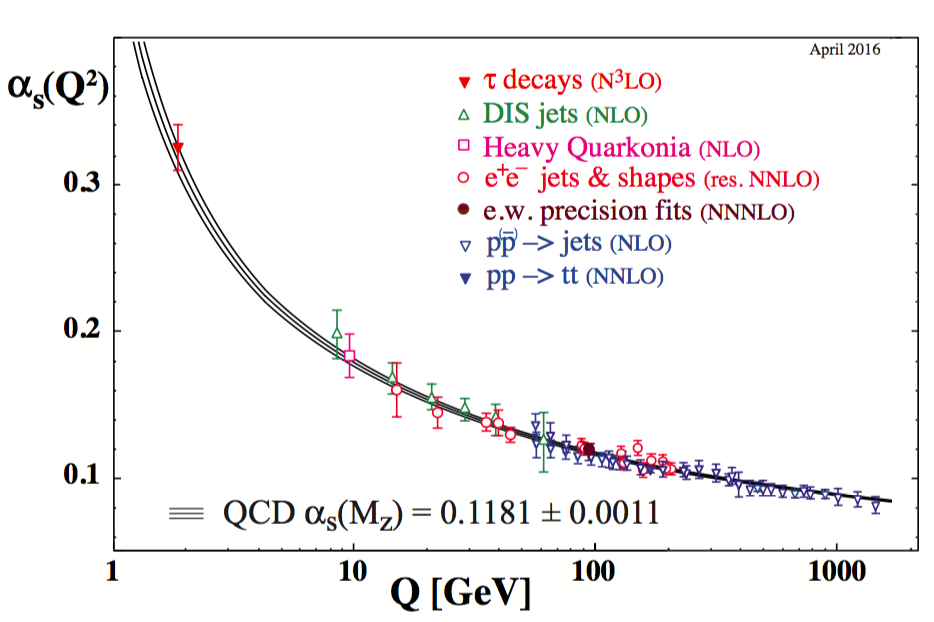
\includegraphics[width=0.6\textwidth]{\chtwo/alphaS_measurement_2016.png}
  \caption{Summary of measurements of the running coupling $\alpha_s$ as a function of the energy scale $Q$ of the process~\cite{Olive:2016xmw}.}
  \label{fig:AlphaS}
\end{figure} 